%%%%%%%%%%%%%%%%%%%%%%%%%%%%%%%%%%%%%%%%%%%%%%%%%%%%%%%%%%%%%%%%%%%%%%%%%%%%%%%
% Author:  Pablo Alvarado
%
% Escuela de Ingeniería Electrónica
% Instituto Tecnológico de Costa Rica
%
% Tesis de Licenciatura
% 
% Phone:   +506 550 2106
% Fax:     +506 591 6629
% email:   palvarado@ietec.org
%
% $Id: main.tex 1513 2010-08-15 01:25:24Z palvarado $
%
%%%%%%%%%%%%%%%%%%%%%%%%%%%%%%%%%%%%%%%%%%%%%%%%%%%%%%%%%%%%%%%%%%%%%%%%%%%%%%%

% \documentclass is book
\documentclass[12pt,twoside,letterpaper]{book}

\usepackage[utf8]{inputenc}
\usepackage{ifthen}                     % provide if-then-else operators

% --------------------------------------------------------------------------
% Global variables required in document formatting
% --------------------------------------------------------------------------
%
% BOOK MODE
%
\newboolean{bookmode}                  % boolean used to control book format
% Ensure that only one of the next two lines is active:
\setboolean{bookmode}{true}           % turn book mode on
%\setboolean{bookmode}{false}           % turn book mode off

%
% DRAFT MODE
%
\newboolean{draftmode}                  % boolean used to control draft-mode
% Ensure that only one of the next two lines is active:
\setboolean{draftmode}{true}            % turn draft mode on
%\setboolean{draftmode}{false}           % turn draft mode off
% --------------------------------------------------------------------------
%
% GENERAL AUTHOR, TITLE AND KEYWORDS
%
% Nombre del Estudiante
\newcommand{\scriptAuthor}{Adrián Ignacio Cervantes Segura}

% Título de la tesis
\newcommand{\scriptTitle}{Unidad de linealización y normalización para un estimador de parámetros de uso en un sistema de optimización de energía en paneles fotovoltaicos} 

% Keywords
\newcommand{\scriptKeywords}{palabras, clave, ...}

% Descripción de la editorial
\newcommand{\boxeditorial}{%
}

% Para el PDF (cambiar si se desea otras cosas a lo indicado arriba
\newcommand{\pdfAuthor}{\scriptAuthor}
\newcommand{\pdfTitle}{\scriptTitle} 
\newcommand{\pdfKeywords}{\scriptKeywords}

% --------------------------------------------------------------------------

% include all packages and define all required general macros
%%%%%%%%%%%%%%%%%%%%%%%%%%%%%%%%%%%%%%%%%%%%%%%%%%%%%%%%%%%%%%%%%%%%%%%%%%%%%%%
% Author:  Pablo Alvarado
%
% Escuela de Electrónica
% Instituto Tecnológico de Costa Rica
%
% Phone:   +506 550 2106
% Fax:     +506 591 6629
% email:   palvarado@ietec.org
%
% $Id: macros.tex 1497 2010-08-09 17:04:26Z palvarado $
%
%%%%%%%%%%%%%%%%%%%%%%%%%%%%%%%%%%%%%%%%%%%%%%%%%%%%%%%%%%%%%%%%%%%%%%%%%%%%%%%

% Configuration of the exercises package, which is used to collect all
% problems and answers in the document.
\usepackage[exercisedelayed,answerdelayed,lastexercise]{exercise}
\renewcounter{Exercise}[chapter]
\renewcommand{\ExerciseName}{Problema}
\renewcommand{\theExercise}{\thechapter.\arabic{Exercise}}
\newcommand{\ExerciseLabel}{Exercise.\theExercise}
\renewcommand{\ExerciseHeader}%
{\textbf{\ExerciseName\ \theExercise.\ \ExerciseHeaderTitle\ }}
\renewcommand{\AnswerHeader}%
{\textbf{\ExerciseName\ \theExercise.\ }}


\usepackage{ifpdf}

% Command to change between draft or release mode:
\newcommand{\ifdraft}[2]{\ifthenelse{\boolean{draftmode}}{#1}{#2}}
% Command to change between draft or release mode:
\newcommand{\ifbook}[2]{\ifthenelse{\boolean{bookmode}}{#1}{#2}}

% include all required packages here
\usepackage[spanish,english]{babel}     % supports english, but default is 
                                        % spanish...
\newcommand*{\SelectSpanish}{%          % well, the last line indeed selects
  \hyphenrules{spanish}%                % english over spanish, but with this
  \languageshorthands{spanish}%         % command we turn it around.
  \captionsspanish                      % The reason: hyperref has some
  \datespanish                          % problems with the spanish babel,
}                                       % so we use some trick here so that it
\AtBeginDocument{\SelectSpanish}        % thinks it is english.

\usepackage{makeidx}                    % to create index file

\ifdraft{%
  %\usepackage[refpage]{nomencl}        % Use to easily administrate the list
 \usepackage{nomencl}                   % of symbols
}{%
 \usepackage{nomencl}
}
%\usepackage{times}                     % replace latex pk fonts with ps type I
                                        % don't forget to use dvips -D600 -Pcmz
                                        % to ensure Type I fonts!
\usepackage{amsmath}
\usepackage{amssymb,amstext}            % AMS-math and symbols package
\usepackage{mathrsfs}                   % Calygraphic fonts for transforms
\usepackage{array}                      % extensions to tabular environment
\usepackage{longtable}                  % supports extraordinary long tables
\usepackage{tabularx}                   % supports tables with fixed width
\usepackage{afterpage}                  % put something only after the page
\usepackage{multirow}                   % supports multiple row grouping in 
                                        % tables
\usepackage{multicol}                   % multiple columns environments
\usepackage{paralist}                   % a few enumeration settings

\usepackage[hang,%
            small,%
            bf]{caption}                % nicer figure captions
%\usepackage{sty/ftcap}                 % switch \abovecaptionskip and
%                                       % \belowcaptionskip for tables, in 
%                                       % order to avoid the caption to be
%                                       % too near to the table itself
% locally added packages
\usepackage{float}                      % really place figures "here" (H)
\usepackage{booktabs}                   % book type tabulars

% the own style with options depending on the draft mode
\ifdraft{%
\usepackage[todo]{sty/tecStyle}         % some command definitions
                                        % options [todo] todo-index
}{%
\usepackage{sty/tecStyle}               % some command definitions
                                        % options [todo] todo-index
}

%% fix the title for examples
\renewcommand{\examplelistname}{Índice de ejemplos}
\renewcommand{\examplename}{Ejemplo}


\usepackage{url}                        % allows linebreaks at certain
                                        % characters or combinations of 
                                        % characters for URLs

\usepackage[nottoc]{tocbibind}          % Fix the hyperrefs to TOC,TOF, etc.
                                        % and ensure that they appear all in 
                                        % the Table of Contents

\usepackage{color}                      % Support for colors
\definecolor{dkred}{rgb}{0.5,0,0}       %   dark red
\definecolor{dkgreen}{rgb}{0,0.3,0}     %   dark green
\definecolor{dkblue}{rgb}{0,0.0,0.5}    %   dark blue
\definecolor{dkgray}{gray}{0.4}         %   dark gray
\definecolor{dkmagenta}{rgb}{0.3,0.0,0.3} % dark magenta
\definecolor{ltyellow}{rgb}{1.0,1.0,0.7}  % light yellow

\newcommand{\bG}[1]{\textcolor{dkgreen}{\textbf{#1}}}
\newcommand{\bR}[1]{\textcolor{dkred}{\textbf{#1}}}
\newcommand{\bB}[1]{\textcolor{dkblue}{\textbf{#1}}}
\newcommand{\bM}[1]{\textcolor{dkmagenta}{\textbf{#1}}}
\newcommand{\bY}[1]{\textcolor{dkyellow}{\textbf{#1}}}
\newcommand{\bC}[1]{\textcolor{dkcyan}{\textbf{#1}}}

% For pdflatex
% - The hyperref package should always be loaded last, since it has to
%   overwrite some of the commands.
% - The package subfigure caused that the pagebackrefs and index refs were set
%   incorrectly.

\ifpdf
%
% final / draft document options
\usepackage[pdftex,final]{graphicx}     % for inserting pdf-graphics.
                                        % options final / draft
\ifdraft{%

\usepackage[pdftex,%
            pdftitle={\pdfTitle},%
            pdfauthor={\pdfAuthor},%
            pdfsubject={Notas de Clase},%
            pdfkeywords={\pdfKeywords},%
            naturalnames=true,
            linktocpage,
            hyperindex,
            colorlinks,
            urlcolor=dkred,          %\href to external url
            filecolor=dkmagenta,     %\href to local file
            linkcolor=dkred,         %\ref and \pageref
            citecolor=dkgreen,       %\cite
            pagecolor=dkred,
            pagebackref,
            plainpages=false,
            pdfpagelabels,
            pdfpagemode=UseOutlines, % means use bookmarks (None,UseOutlines)
            % bookmarksopen=false,   % would show the whole hierarchy if true
            bookmarksnumbered=true,
            pdfpagelayout=OneColumn, % SinglePage,OneColumn,TwoColumnLeft,...
            pdfview=FitH, % FitB,FitBH,FitBV,Fit,FitH,FitV
            pdfstartview=FitH, % FitB,FitBH,FitBV,Fit,FitH,FitV
            ]{hyperref}
}{%
\usepackage[pdftex,%
            pdftitle={\pdfTitle},%
            pdfauthor={\pdfAuthor},%
            pdfsubject={Notas de clase},%
            pdfkeywords={\pdfKeywords},%
            naturalnames=true,
            linktocpage,hyperindex,
            colorlinks,
            urlcolor=dkred,          %\href to external url
            filecolor=dkmagenta,     %\href to local file
            linkcolor=dkred,         %\ref and \pageref
            citecolor=dkgreen,       %\cite
            pagecolor=dkred,
            % pagebackref,           % only in draft modus should this be on.
            plainpages=false,
            pdfpagelabels,
            pdfpagemode=UseOutlines, % means use bookmarks (None,UseOutlines)
            % bookmarksopen=false,   % open the whole hierarchy if true!
            bookmarksnumbered=true,
            pdfpagelayout=OneColumn, % SinglePage,OneColumn,TwoColumnLeft,...
            pdfview=FitH, % FitB,FitBH,FitBV,Fit,FitH,FitV
            pdfstartview=FitH, % FitB,FitBH,FitBV,Fit,FitH,FitV
            ]{hyperref}
}

%
% Ensure that the links of the images point to the top of the images and not
% to the caption
%
\usepackage[figure]{hypcap}

% %
% % Ensure that pdfLaTeX do the same spacing as LaTeX
% %
\pdfadjustspacing=1 
% %
\else   % i.e. if not pdf

\usepackage[active]{srcltx}             % insert links into the dvi to jump
\usepackage[dvips,final]{graphicx}      % for inserting eps-graphics.
                                        % options final / draft
                                        % into the sources directly.
\ifdraft{%
\usepackage[ps2pdf,%
            pdftitle={\pdfTitle}%
            pdfauthor={\pdfAuthor},%
            pdfsubject={Notas de clase},%
            pdfkeywords={\pdfKeywords},%
            % plainpages=false,
            linktocpage,
            hyperindex,
            pagebackref,
            % pdfpagelabels,
            pdfpagemode=UseOutlines,
            pdfstartview=FitH]{hyperref}
}{%
\usepackage[ps2pdf,%
            pdftitle={\pdfTitle}%
            pdfauthor={\pdfAuthor},%
            pdfsubject={Notas de clase},%
            pdfkeywords={\pdfKeywords},%
            % plainpages=false,
            linktocpage,
            hyperindex,
            % pagebackref,
            % pdfpagelabels,
            pdfpagemode=UseOutlines,
            pdfstartview=FitH]{hyperref}
}

%\usepackage[ps2pdf]{hyperref}

\fi  % end of if pdf or not

\usepackage{sty/algorithmic}            % algorithmic environment


\usepackage{rotating}                   % allow block rotation


%%%%%%%%%%%%%%%%%%%%%%%%%%%%%%%%%%%%%%%%%%%%%%%%%%%%%%%%%%%%%%%%%%%%%%%%%%%%%%%

%\sloppy

%
% Some own font definitions
%
\DeclareMathAlphabet{\mathpzc}{OT1}{pzc}{m}{it}
\DeclareMathAlphabet{\mathpss}{OT1}{cmss}{m}{sl}

%
% page layout
%

\usepackage{vmargin}
\setpapersize{USletter}

% For letter-paper printing
\setmarginsrb{33mm}{8mm}{23mm}{7mm}{15pt}{15pt}{7mm}{12mm}
%\setlength{\headheight}{15pt}         % fancy headers wanted this

%
% Fraction of Float Object / Text
%

\renewcommand{\topfraction}{0.95}       % how much of top of page should be 
                                        % allowed to be float object?
\renewcommand{\bottomfraction}{0.95}    % how much of bottom of page should be
                                        % allowed to be float object?
\renewcommand{\textfraction}{0.05}      % how much of page must be text?

\usepackage{fancyhdr}                   % fancy page headers

\usepackage{lastpage}

%
% header and footer layout (needs package fancyhdr)
%
\newcommand{\copyrightfooter}{\tiny{\copyright 2005-2010 --- P.~Alvarado %
    \qquad Uso exclusivo ITCR}}
%
\newcommand{\draftfoot}%
  {\ifdraft{\textcolor{dkblue}{\tiny\textsl{Borrador: \today}}{}}
           {}
}

\pagestyle{fancy}
\renewcommand{\chaptermark}[1]{\markboth{{\small
    \thechapter\hspace*{1mm}#1}}{}}
\renewcommand{\sectionmark}[1]{\markright{{\small
    \thesection\hspace*{1mm}#1}}{}}
\lhead[{\small\textbf\thepage}]{\fancyplain{}%
        {{\slshape \small\nouppercase{\leftmark}}}}
\chead[]{}
\rhead[\fancyplain{}%
        {{\slshape \small\nouppercase{\rightmark}}}]{{\small\textbf\thepage}}
\lfoot[]{\draftfoot}
\ifbook{%
  \cfoot[]{}
}{
  \cfoot[\copyrightfooter]{\copyrightfooter}
}
\rfoot[\draftfoot]{}
\renewcommand{\headrulewidth}{0.5pt}
\renewcommand{\footrulewidth}{0pt}

%
% Caption style for tables
% Requires the packages caption2 and ftcap
% (caption2 required this, but is obsolete now:)
%
%\newcaptionstyle{tablecaptionstyle}{%
%  \renewcommand\captionlabelfont{\normalsize\bf}
%  \renewcommand\captionfont{\normalsize}
%  \usecaptionstyle{hang}%
%}

% For caption v3:
\captionsetup[table]{position=top,format=hang,textfont={normalsize},labelfont={normalsize,bf}}

\newcommand{\tablecaption}[2][foo]{%
  \ifthenelse{\equal{#1}{foo}}{%
    %\captionstyle{tablecaptionstyle}%
    \caption{#2}%
  }
  {%
    %\captionstyle{tablecaptionstyle}%
    \caption[#1]{#2}%
  }
}
\addto\extrasspanish{\renewcommand{\tablename}{Tabla}}
\addto\extrasspanish{\renewcommand{\listtablename}{\'Indice de tablas}}

%
% paragraph layout
%
\renewcommand{\baselinestretch}{1.1}    % line spacing
\parindent0em                           % indentation width of first line
\parskip1.3ex                           % space between paragraphs

%
% document consists of
% chapter - section - subsection - subsubsection - paragraph - subparagraph
%
\setcounter{secnumdepth}{2}             % depth of section numbering
\setcounter{tocdepth}{2}                % depth of table of contents

%
% prepares index from entries like \index{word} or \index{group!word}.
% don't forget to call "makeindex filename" for final index generation.
%
\makeindex                            %% for package makeidx.sty
%\newindex{default}{idx}{ind}{Index}  %% for package index.sty

\newcommand{\octave}{GNU/Octave}


%
% prepares notation or nomenclature 
%
%\makeglossary
\makenomenclature

%%% Local Variables: 
%%% mode: latex
%%% TeX-master: "main"
%%% End: 


% allow equations to be splitted (breaked) into several pages
\allowdisplaybreaks[3]

% --------------------------------------------------------------------------
\begin{document}
  % where to look for graphics
  \graphicspath{{./}{./fig/}}
  %\graphicspath{C:/Users/Adrian Cervantes/Desktop/tesis_latex_template/fig}

  \pagenumbering{alph}
  % fix some terms not activated due to the bug of hyperref with spanish.
  \renewcommand{\tablename}{Tabla}
  \renewcommand{\listtablename}{\'Indice de tablas}
  \renewcommand{\examplesolution}{Solución}
  \pagestyle{empty}

  %% ---------------------------------------------------------------------------
%% titlepage.tex
%%
%% Title page
%%
%% $Id: titlepage.tex 1452 2010-07-07 00:55:16Z palvarado $
%% ---------------------------------------------------------------------------

\thispagestyle{empty} 

\begin{center}

Tecnológico de Costa Rica

\par\vspace{1ex}

Escuela de Ingeniería Electrónica

\par\vspace{20mm}



\includegraphics[width=100mm]{./TEC.jpg}

\par\vspace*{\fill}

{\large\bf{\scriptTitle}}

\par\vspace*{\fill}

Informe de Proyecto de Graduación para optar por el título de

Ingeniero en Electrónica con el grado académico de Licenciatura

\par\vspace{20mm}

\scriptAuthor

\vspace*{\fill}

\ifdraft{%
{Borrador de \today}
}{
Cartago, 19 de noviembre, 2010
}
\end{center}
\newpage 
\cleardoublepage 


%%% Local Variables: 
%%% mode: latex
%%% TeX-master: "main"
%%% End: 
                                 % Titlepage
  \thispagestyle{empty}

\rule{10mm}{0pt}

\vfill

Declaro que el presente Proyecto de Graduación ha sido realizado enteramente
por mi persona, utilizando y aplicando literatura referente al tema e
introduciendo conocimientos propios.

En los casos en que he utilizado bibliografía he procedido a indicar las
fuentes mediante las respectivas citas bibliográficas.  En consecuencia,
asumo la responsabilidad total por el trabajo de graduación realizado y por
el contenido del correspondiente informe final.



\vspace*{8mm}

\begin{flushright}
  \scriptAuthor\par
  Cartago, \today\par
  Céd: 1-1508-0317
\end{flushright}

\cleardoublepage

%%% Local Variables: 
%%% mode: latex
%%% TeX-master: "main"
%%% End: 

  \thispagestyle{empty}

%%
%% Indique los nombres de los lectores y asesor
\newcommand{\lectorI}{Dra.\, María del Pilar Pérez Fernández}
\newcommand{\lectorII}{Dr.\,Juan Pérez Hernández}
\newcommand{\director}{Dr.\,Pablo Alvarado Moya}
%% Revise además que 


\begin{center}
  \begin{tabular}{c}
    Instituto Tecnológico de Costa Rica \\
    Escuela de Ingeniería Electrónica \\
    Proyecto de Graduación \\
    Tribunal Evaluador
  \end{tabular}
\end{center}

\vfill

Proyecto de Graduación defendido ante el presente Tribunal Evaluador como 
requisito para optar por el título de Ingeniero en Electrónica con el grado 
académico de Licenciatura, del Instituto Tecnológico de Costa Rica.  

\vfill

\vspace*{20mm}
\begin{center}
 Miembros del Tribunal
\end{center}
\vspace*{8mm}

\vfill

\begin{center}
  \begin{tabular}{ccc}
    \rule{70mm}{0.5pt} & \rule{15mm}{0pt} & \rule{70mm}{0.5pt} \\
    \lectorI && \lectorII \\
    Profesora Lectora && Profesor Lector
  \end{tabular}
  
  \vspace{10mm}

  \begin{tabular}{c}
    \rule{6cm}{0.5pt} \\
    \director \\
    Profesor Asesor
  \end{tabular}
\end{center}

\vfill


Los miembros de este Tribunal dan fe de que el presente trabajo de graduación
ha sido aprobado y cumple con las normas establecidas por la Escuela de
Ingeniería Electrónica.

\vfill

\begin{center}
  Cartago, 29 de noviembre de 2011\par
\end{center}

\cleardoublepage

%%% Local Variables: 
%%% mode: latex
%%% TeX-master: "main"
%%% End: 

  \thispagestyle{empty}

%%
%% Los nombres de lectores y asesor se definen en el archivo tribunal.tex
%%

\begin{center}
  \begin{tabular}{c}
    Instituto Tecnológico de Costa Rica \\
    Escuela de Ingeniería Electrónica \\
    Proyecto de Graduación \\
    Tribunal Evaluador \\
    Acta de Evaluación
  \end{tabular}
\end{center}

\vfill

Proyecto de Graduación defendido ante el presente Tribunal Evaluador como 
requisito para optar por el título de Ingeniero en Electrónica con el grado 
académico de Licenciatura, del Instituto Tecnológico de Costa Rica.  

\vspace*{15mm}

\begin{center}
  Estudiante: Adrián Ignacio Cervantes Segura
\end{center}

\vfill

\begin{center}
  Nombre del Proyecto: \emph{Unidad de linealización y normalización para un estimador de parámetros de uso en un sistema de optimización de energía en paneles fotovoltaicos}
\end{center}

\vspace*{20mm}
\begin{center}
 Miembros del Tribunal
\end{center}
\vspace*{8mm}

\vfill

\begin{center}
  \begin{tabular}{ccc}
    \rule{70mm}{0.5pt} & \rule{15mm}{0pt} & \rule{70mm}{0.5pt} \\
    \lectorI && \lectorII \\ %% Nombres definidos en tribunal.tex
    Profesora Lector && Profesor Lector
  \end{tabular}
  
  \vspace{10mm}

  \begin{tabular}{c}
    \rule{6cm}{0.5pt} \\
    \director \\ %% Definido en tribunal.tex
    Profesor Asesor
  \end{tabular}
\end{center}

\vfill

Los miembros de este Tribunal dan fe de que el presente trabajo de graduación
ha sido aprobado y cumple con las normas establecidas por la Escuela de
Ingeniería Electrónica.

\vfill

\begin{center}
  Nota final del Proyecto de Graduación: \rule{3cm}{0.5pt}
\end{center}
\vfill

\begin{center}
  Cartago, 25 de marzo de 2016\par
\end{center}

\cleardoublepage

%%% Local Variables: 
%%% mode: latex
%%% TeX-master: "main"
%%% End: 

  \chapter*{Resumen}
\thispagestyle{empty}

En esta tesis se presenta el diseño de un linealizador de corriente descrito en lenguaje VHDL, basado en el estándar para aritmética de coma flotante de IEEE 754 para microprocesadores, para el cual se utiliza el formato binario de precisión simple de 32 bits, utilizando el algoritmo de CORDIC para realizar la operación logaritmo natural. Por otro lado se realiza un convertidor de formato IEEE 754 coma flotante a coma fija, ambos en 32 bits, por último se normaliza el dato en coma fija, esta normalización se aplica tanto en corriente como en tensión. Estos circuitos serán utilizados en un sistema de aumento de eficiencia para suministros de paneles fotovoltaicos. Este linealizador cuenta con la capacidad para realizar operaciones aritméticas en coma flotante, lo cual es fundamental para una mejor precisión y desempeño del sistema en el procesamiento de los datos, ha sido diseñado considerando los parámetros de velocidad, área utilizada dentro de la FPGA y consumo de potencia estimada, además el circuito ha sido sintetizado y simulado sobre la FPGA Virtex® 7 de la familia Xilinx®. El circuito se interconectó en un diagrama esquemático principal para mayor facilidad de incorporación de los bloques de control, entradas y salidas.
 

\bigskip

\textbf{Palabras clave:} Aritmética Binaria, Formato IEEE 754, coma fija, FPGA, VHDL.





\clearpage
\chapter*{Abstract}
\thispagestyle{empty}

This thesis presents the design of a current linearizer described in VHDL language based on the standard for Arithmetic floating Point IEEE-754 for microprocessors and the binary format used is single-precision 32-bit, using CORDIC algorithm to perform the operation. On the other hand a converter IEEE 754 floating point to fixed point, both in 32 bits, finally the data is normalized in fixed point, this normalization is applied to both current and voltage. These circuits will be used in a system for  increased efficiency of supplies photovoltaic panels. This linearizer has the ability to perform arithmetic floating point operations, which is critical for better accuracy and performance of the system in data processing, it has been designed considering the parameters of speed, area used within the FPGA and consumption estimated power addition the circuit has been synthesized and simulated on FPGA Xilinx® Virtex® 7 family. The circuit has been interconnected in a main schematic diagram for easy incorporation of control blocks, inputs, outputs.


\bigskip

\textbf{Keywords:} Binary arithmetic, IEEE 754 Format, Fixed point, FPGA, VHDL. 

%\cleardoublepage

%%% Local Variables: 
%%% mode: latex
%%% TeX-master: "main"
%%% End: 

  \vspace*{0.4\textheight}
{\hfill{\Large{\emph{a mis queridos padres}}}}

  \chapter*{Agradecimientos}
\thispagestyle{empty}

En primer lugar a Dios, quién me ha dado sabiduría y ha sido un pilar importante a lo largo de esta carrera. 

Al Ing. Alfonso Chacón Rodríguez, quién ha sido un gran apoyo en el desarrollo del proyecto y en cursos a lo largo de la carrera, por los consejos, paciencia, conocimiento compartido y su nivel de profesionalismo. 


A mi familia, por apoyarme a lo largo de toda mi educación, por la ayuda y por los grandes sacrificios que ha hecho para poder llegar donde estoy hoy, por los valores y por toda la ayuda que me han dado en todos estos años.


Finalmente, agradezco a las personas que de una u otra forma me han apoyado a lo largo del proceso.
\vspace*{1cm}

\scriptAuthor

Cartago, \today

\cleardoublepage

%%% Local Variables: 
%%% mode: latex
%%% TeX-master: "paMain"
%%% End: 


  %----------------------------------------------------------------------------
  \frontmatter
  %----------------------------------------------------------------------------
  \pagestyle{fancy}

  \pdfbookmark[1]{Indice General}{Indice General}

  \parskip0ex                           % space between paragraphs

  \tableofcontents                                      % Table of contents
  \listoffigures                                        % List of figures
  \listoftables                                         % List of tables

\ifdraft{%
  % todo's                                              % TODOs
  %\listoftodo %pagrevisar
}{%
}

  %% ---------------------------------------------------------------------------
%% paNotation.tex
%%
%% Notation
%%
%% $Id: notation.tex 1467 2010-07-24 16:47:17Z palvarado $
%% ---------------------------------------------------------------------------

\newcommand{\nms}{\negmedspace}

%%
% Commands required for the nomenclature groups
%
% There are following prefix forms:
%  a   abbreviation    \syma[key]{symbol}{description}
%  g   general         \symg[key]{symbol}{description}
%%

\newcommand{\nmstyle}[1]{\large\item[\textbf{#1}]\normalsize}

\renewcommand{\nomgroup}[1]{%
  \ifthenelse{\equal{#1}{A}}{\nmstyle{Abreviaciones}\normalsize}{%
  \ifthenelse{\equal{#1}{G}}{\bigskip\nmstyle{Notación general}\normalsize}%
  }
}

\newcommand{\syma}[3][foo]{%
  \ifthenelse{\equal{#1}{foo}}%
  {\nomenclature[A#2\ ]{#2}{#3}}{\nomenclature[A#1\ ]{#2}{#3}}}
\newcommand{\symg}[3][foo]{%
  \ifthenelse{\equal{#1}{foo}}%
  {\nomenclature[G#2\ ]{#2}{#3}}{\nomenclature[G#1\ ]{#2}{#3}}}

%%
% Command definitions for localized symbol format definition
%%
\renewcommand{\Re}{\operatorname{Re}}
\renewcommand{\Im}{\operatorname{Im}}

\newcommand{\prt}[1]{\ensuremath{\mathcal{#1}}}         %% partitioning
\newcommand{\img}[1]{\ensuremath{\mathcal{#1}}}         %% image as a set
\newcommand{\reg}[1][R]{\ensuremath{\mathcal{#1}}}      %% region
\newcommand{\pred}[1]{\ensuremath{\mathrm{#1}}}         %% predicate
\newcommand{\operat}[2]{\mathcal{#1}\left\{#2\right\}}
\newcommand{\transf}[1]{\mathscr{#1}}
\newcommand{\fourier}[1]{\transf{F}\left\{#1\right\}}
\newcommand{\ifourier}[1]{\transf{F}^{-1}\left\{#1\right\}}
\newcommand{\laplace}[1]{\transf{L}\left\{#1\right\}}
\newcommand{\ulaplace}[1]{\transf{L}_u\left\{#1\right\}}
\newcommand{\blaplace}[1]{\transf{L}_b\left\{#1\right\}}
\newcommand{\ilaplace}[1]{\transf{L}^{-1}\left\{#1\right\}}
\newcommand{\ztrans}[1]{\transf{Z}\left\{#1\right\}}
\newcommand{\iztrans}[1]{\transf{Z}^{-1}\left\{#1\right\}}
\newcommand{\zutrans}[1]{\transf{Z}_u\left\{#1\right\}}
\newcommand{\exceq}{\ensuremath{\overset{!}{=}}}

\newcommand{\signum}{\operatorname{signum}}
\newcommand{\vct}[1]{\ensuremath{\underline{\mathbf{#1}}}}
\newcommand{\mat}[1]{\ensuremath{\mathbf{#1}}}
\newcommand{\vctmu}{\vct{\boldsymbol{\mu}}}
\newcommand{\vctzeta}{\vct{\boldsymbol{\zeta}}}
\newcommand{\vctpi}{\vct{\boldsymbol{\pi}}}
\newcommand{\vctvarphi}{\vct{\boldsymbol{\varphi}}}
\newcommand{\raum}[1]{\ensuremath{\mathbb{#1}}}
\newcommand{\matSigma}{\mat{\boldsymbol{\Sigma}}}
\newcommand{\matLambda}{\mat{\boldsymbol{\Lambda}}}
\newcommand{\matPsi}{\mat{\boldsymbol{\Psi}}}
\newcommand{\matPhi}{\mat{\boldsymbol{\Phi}}}
\newcommand{\row}[2]{\ensuremath{\mathbf{\underline{#1}_{#2(\cdot)}}}}
\newcommand{\col}[2]{\ensuremath{\mathbf{\underline{#1}_{(\cdot) #2}}}}
\newcommand{\seq}[1]{\ensuremath{#1}}
\newcommand{\set}[1]{\ensuremath{\mathcal{#1}}}
\newcommand{\gset}[1]{\ensuremath{#1}} %% set for greek symbols
\newcommand{\front}[1]{\widehat{\set{#1}}}
\newcommand{\setlambda}{\set{\boldsymbol{\lambda}}}
\newcommand{\klass}[1]{\ensuremath{\mathpss{#1}}}
\newcommand{\graph}[1]{\ensuremath{\mathsf{#1}}}
\newcommand{\lab}[1]{\ensuremath{\mathpss{L}(#1)}}
\newcommand{\myfrac}[2]{{\footnotesize #1/#2}}
\newcommand{\ifthenspc}{\rule{3mm}{0mm}}
\newcommand{\point}[1]{\ensuremath{\mathsf{#1}}}
\newcommand{\estim}[1]{\ensuremath{\hat{#1}}}
\newcommand{\numset}[1]{\ensuremath{\mathbb{#1}}}
\newcommand{\tuple}[1]{\ensuremath{\left\langle#1\right\rangle}}
\newcommand{\conj}[1]{\ensuremath{{{#1}^{\ast}}}}
\newcommand{\base}[1]{\set{#1}}
\newcommand{\zeron}[1]{\ensuremath{\underset{\uparrow}{#1}}}
\newcommand{\sysT}{\ensuremath{\mathcal{T}}}
\newcommand{\sys}[1]{\ensuremath{\sysT\left[#1\right]}}
\newcommand{\sen}{\operatorname{sen}} % sinus in spanish (seno)
\newcommand{\senh}{\operatorname{senh}} % sinus hiperbolicus in spanish (seno)
\newcommand{\arcsen}{\operatorname{arcsen}} % arcus sinus hiperbolicus in spanish (arcoseno)
\newcommand{\sgn}{\operatorname{sgn}} % signus
\newcommand{\roc}{\text{ROC: }}

\newcommand{\code}[1]{\texttt{#1}}
\newcommand{\conv}{\ensuremath{\ast}}
\newcommand{\cconv}{\ensuremath{\;\,\text{\footnotesize{N}}\!\!\!\!\!\!\bigcirc}}
\newcommand{\Ln}{\operatorname{Ln}}
\newcommand{\sa}{\operatorname{sa}}
\newcommand{\senc}{\operatorname{senc}}
\newcommand{\si}{\operatorname{si}}


%% Natural, Integer and Real Numbers
\newcommand{\setA}{\ensuremath{\mathbb{A}}}
\newcommand{\setB}{\ensuremath{\mathrm{I\negthinspace B}}}
\newcommand{\setC}{\ensuremath{\mathbb{C}}}
\newcommand{\setD}{\ensuremath{\mathrm{I\negthinspace D}}}
\newcommand{\setE}{\ensuremath{\mathrm{I\negthinspace E}}}
\newcommand{\setF}{\ensuremath{\mathrm{I\negthinspace F}}}
\newcommand{\setG}{\ensuremath{\mathbb{G}}}
\newcommand{\setH}{\ensuremath{\mathrm{I\negthinspace H}}}
\newcommand{\setI}{\ensuremath{\mathbb{I}}}
\newcommand{\setJ}{\ensuremath{\mathbb{J}}}
\newcommand{\setK}{\ensuremath{\mathrm{I\negthinspace K}}}
\newcommand{\setL}{\ensuremath{\mathrm{I\negthinspace L}}}
\newcommand{\setM}{\ensuremath{\mathrm{I\negthinspace M}}}
\newcommand{\setN}{\ensuremath{\mathrm{I\negthinspace N}}}
\newcommand{\setO}{\ensuremath{\mathbb{O}}}
\newcommand{\setP}{\ensuremath{\mathrm{I\negthinspace P}}}
\newcommand{\setQ}{\ensuremath{\mathbb{Q}}}
\newcommand{\setR}{\ensuremath{\mathrm{I\negthinspace R}}}
\newcommand{\setS}{\ensuremath{\mathbb{S}}}
\newcommand{\setT}{\ensuremath{\mathbb{T}}}
\newcommand{\setU}{\ensuremath{\mathbb{U}}}
\newcommand{\setV}{\ensuremath{\mathbb{V}}}
\newcommand{\setW}{\ensuremath{\mathbb{W}}}
\newcommand{\setX}{\ensuremath{\mathbb{X}}}
\newcommand{\setY}{\ensuremath{\mathbb{Y}}}
\newcommand{\setZ}{\ensuremath{\mathbb{Z}}}


%%
% Multimap symbols
%
\newcommand{\ttoF}{\,\circ\!\negthickspace\longrightarrow\negthickspace\!\negthickspace\bullet\,}
\newcommand{\Ftot}{\,\bullet\negthickspace\!\negthickspace\longleftarrow\!\negthickspace\circ\,}
\newcommand{\ttoZ}{\ttoF}
\newcommand{\Ztot}{\Ftot}
\newcommand{\ttoZu}{\overset{z_u}{\ttoF}}
\newcommand{\Zutot}{\overset{z_u}{\Ftot}}
\newcommand{\vttoF}{\text{\begin{sideways}$\Ftot$\end{sideways}}}
\newcommand{\vFtot}{\text{\begin{sideways}$\ttoF$\end{sideways}}}
\newcommand{\vttoZ}{\vttoF}
\newcommand{\vZtot}{\vFtot}
\newcommand{\ttoDF}{\underset{N}{\ttoF}}
\newcommand{\DFtot}{\underset{N}{\Ftot}}

\newcommand{\thisis}[2]{\underset{#1}{\underbrace{#2}}}

%%% Local Variables:
%%% mode: latex
%%% TeX-master: "paMain"
%%% End:
                                    % Notation
  %% ---------------------------------------------------------------------------
%% paNotation.tex
%%
%% Notation
%%
%% $Id: paNotation.tex,v 1.15 2004/03/30 05:55:59 alvarado Exp $
%% ---------------------------------------------------------------------------

\cleardoublepage
\renewcommand{\nomname}{Lista de símbolos y abreviaciones}
\markboth{\nomname}{\nomname}
\renewcommand{\nompreamble}{\addcontentsline{toc}{chapter}{\nomname}%
\setlength{\nomitemsep}{-\parsep}
\setlength{\itemsep}{10ex}
}

%%
% Símbolos en la notación general
% (es posible poner la declaración en el texto
%%

\symg[t]{$\sys{\cdot}$}{Transformación realizada por un sistema}
\symg[yscalar]{$y$}{Escalar.}
\symg[zconjugado]{$\conj{z}$}{Complejo conjugado de $z$}
\symg[rcomplexreal]{$\Re(z)$ o $z_{\Re}$}{Parte real del número complejo $z$}
\symg[icompleximag]{$\Im(z)$ o $z_{\Im}$}{Parte imaginaria del número
                                        complejo $z$}
\symg[jimaginario]{$j$}{$j=\sqrt{-1}$}
\symg[xvector]{$\vct{x}$}{Vector. \newline\hspace{1mm}%
  $\vct{x}=\left[ x_1 \; x_2 \; \ldots \; x_n \right]^T =
  \begin{bmatrix}
    x_1 \\ x_2 \\ \vdots \\ x_n
  \end{bmatrix}$}

\symg[amatrix]{$\mat{A}$}{Matriz. \newline\hspace{1mm}%
  $\mat{A} =
  \begin{bmatrix}
    a_{11} & a_{12} & \cdots & a_{1m}\\
    a_{21} & a_{22} & \cdots & a_{2m}\\
    \vdots & \vdots & \ddots & \vdots\\
    a_{n1} & a_{n2} & \cdots & a_{nm}\\
  \end{bmatrix}$}

\symg[C]{$\setC$}{Conjunto de los números complejos.}

%%
% Algunas abreviaciones
%%

\syma{PCA}{Análisis de componentes principales}
\syma{WSN}{Redes Inalámbricas de Sensores}
\syma{ASM}{Modelos Activos de Forma}

\printnomenclature[20mm]

%%% Local Variables:
%%% mode: latex
%%% TeX-master: "paMain"
%%% End:
                                    % Abbreviation

  \parskip1.3ex                           % space between paragraphs

  %----------------------------------------------------------------------------
  \mainmatter
  %----------------------------------------------------------------------------
  % where to look for graphics
  \graphicspath{{./}{./fig/}}

  % Main files
  %% ---------------------------------------------------------------------------
%% intro.tex
%%
%% Introduction
%%
%% $Id: intro.tex 1477 2010-07-28 21:34:43Z palvarado $
%% ---------------------------------------------------------------------------

\chapter{Introducción}
\label{chp:intro}

En la \nt{introducción} deben quedar completamente claros los siguientes
aspectos, cuyo significado depende del tipo concreto de tesis:

\begin{compactitem}
\item Contexto
\item Problema
\item Esbozo de solución
\item Objetivos y estructura
\end{compactitem}

El contexto corresponde al entorno donde se desarrolla el proyecto, que puede
ser el área general de aplicación, un dominio de problemas, etc. El problema
concreto se sintetiza usualmente en una frase o pregunta. Esta pregunta debería
ser una consecuencia a la que se llega después de realizar el desarrollo del
contexto. Del planteamiento del problema se deriva cuál es el objetivo del
trabajo en particular, que a su vez debe conducir al lector de forma natural al
esbozo de la solución del problema a tratar en la tesis. Generalmente para
aclarar la solución se hace uso de un diagrama de bloques o diagrama de flujo
general, es decir, desde un nivel de abstracción alto, donde no sea necesario
entrar en detalles técnicos. Usualmente este diagrama y su breve explicación
dictan cuál debe ser la estructura del resto del tesis, que es mencionada
siempre al final de la introducción.

Una buena introducción debe lograr que el lector tenga interés de leer el resto
del tesis.

Es recomendable dividir la tesis en secciones, nombradas cada una de acuerdo a
su contenido. \textbf{Jamás} utilice los nombres de la guía como
``\emph{Problema existente e importancia de su solución}'', sino algo como ``La
deforestación en Costa Rica'' o lo que se adecúe a su problema en particular.

Recuerde que en español solo la primera letra del título va en mayúscula
(exceptuando nombres propios, por supuesto).

\section{Objetivos y estructura del documento}

\index{objetivos}
Esta plantilla LaTeX tiene como objetivo simplificar la construcción del
documento de tesis, presentando ejemplo de figuras y tablas, así como otorgar
una plataforma de compilación en GNU/Linux que simplifique la administración de
todo el documento.

La última sección de la introducción usualmente sí tiene un título estandar que
es ``Objetivos y estructura del documento'', donde se presentan \emph{en prosa}
los objetivos general y específicos que ha tenido el proyecto de graduación,
así como la estructura de la tesis (por ejemplo, ``en el siguiente capítulo se
esbozan los fundamentos teóricos necesarios para explicar en el
capítulo~\ref{ch:solucion} la propuesta realizada$\ldots$''

%%% Local Variables: 
%%% mode: latex
%%% TeX-master: "main"
%%% End: 

  \chapter{Marco teórico}
\label{ch:marco}

\section{Descripción}

En un sistema de paneles fotovoltaicos es de suma importancia la eficiencia energética, para esto se debe estudiar el funcionamiento, curvas características, parámetros para poder caracterizar un panel, el modelo matemático tanto el ideal como la aproximación real, ecuaciones características obtenidas a partir de cada modelo, características del sistema que se requiere optimizar, algoritmos de calculo para realizar operaciones que se requieren en la solución, entre otros.

\section{Panel Fotovoltaico}

Las celdas solares se pueden describir como una junta \nt{p-n}, por medio de la radiación electromagnética proveniente del sol que incide sobre la capa de semiconductor, esta se transforma en el electricidad por un efecto fotovoltaico, en donde los fotones al tener mayor energía que la banda prohibida del semiconductor crean un par electrón-hueco, el campo eléctrico que se ejerce en la junta \nt{p-n} mueve los electrones (\nt{portadores}) lo que produce una fotocorriente, esta es directamente proporcional a la radiación del sol. Debido al proceso de fabricación del panel, posee un comportamiento exponencial y no lineal muy similar al de un diodo [1]. 

\subsection{Curvas Corriente-Tensión(I-V) para un PV }

\begin{figure}[H]
  \centering
    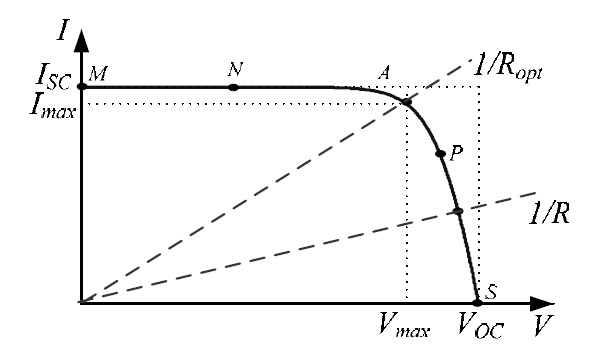
\includegraphics[scale=0.6]{./IV.jpg}
    \rule{35em}{0.5pt}
  \caption[Curva Corriente(A)-Tensión(V)]{Curva Corriente(A)-Tensión(V) }
  \label{fig:Curva_PV}
\end{figure}

La curva característica de un PV  se puede obtener manteniendo fijos los parámetros de irradiancia(S) y temperatura(T) esto bajo condiciones controladas, si se tiene una carga en las terminales de salida, la potencia entregada solo dependerá del valor de la carga, de manera que si la carga es pequeña (puntos M-N) el panel se comportará como una fuente de corriente, pero si la carga es grande(puntos PS) se comportará como una fuente de tension[2]. 

Dentro de la caracterización de la celda se realizan varias pruebas: 

\begin{compactitem}

\item \nt{Corriente de corto circuito $\ I_{sc}$ }: Se define como el valor máximo de la corriente generada por el panel, en condiciones de cortocircuito $\ V=0$.


\item \nt{Tensión de circuito abierto $\ V_{oc}$}: Se define como el valor que se tiene en la junta \nt{p-n} cuando se tiene una corriente generada $\ I=0$.

\item  \nt{Punto de máxima potencia}: se puede observar en el punto A$\left(V_{max},I_{max} \right)$ de la figura \ref{fig:Curva_PV} donde la potencia máxima de la carga resistiva es $\ P_{max} = V_{max}I_{max}$


\end{compactitem}



\subsection{Modelos del panel fotovoltaico}

Un panel fotovoltaico se puede modelar de manera simple (ideal), utilizando una fuente de corriente en paralelo con un diodo, la corriente de salida sera proporcional al radiación sobre la celda (foto-corriente)

\begin{figure}[H]
  \centering
    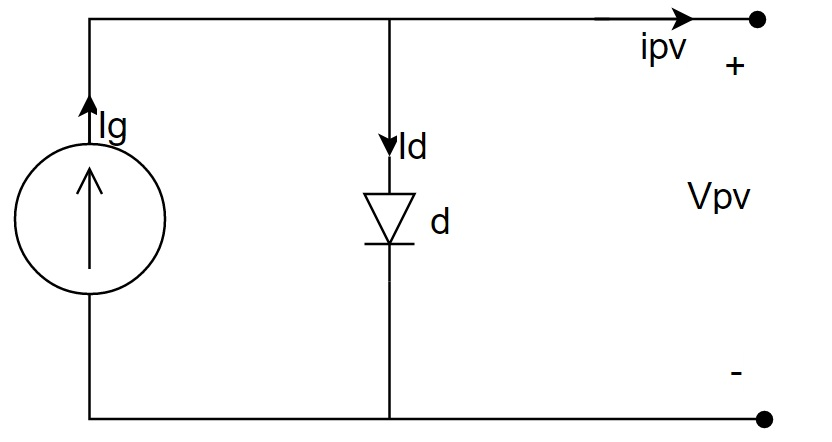
\includegraphics[scale=0.5]{./M1PV.jpg}
    \rule{35em}{0.5pt}
  \caption[Modelo simple ideal para un PV]{ Modelo simple ideal para un PV}
  \label{fig:Modelo1_PV}
\end{figure}

La figura \ref{fig:Modelo1_PV} muestra el modelo básico, sin embargo este se puede realizar de una manera mas compleja, agregando variables para las características del panel: 

\begin{compactitem}

\item Dependencia de la Temperatura, la corriente de saturación del diodo (\nt{Is}) y la foto corriente (\nt{Ig})


\item Perdidas debidas al flujo de corriente (\nt{Rs}) y perdidas con referencia a tierra (\nt{Rp}).

\item  Un parámetro \nt{n} que será el numero de celdas en análisis. 

\end{compactitem}

\begin{figure}[H]
  \centering
    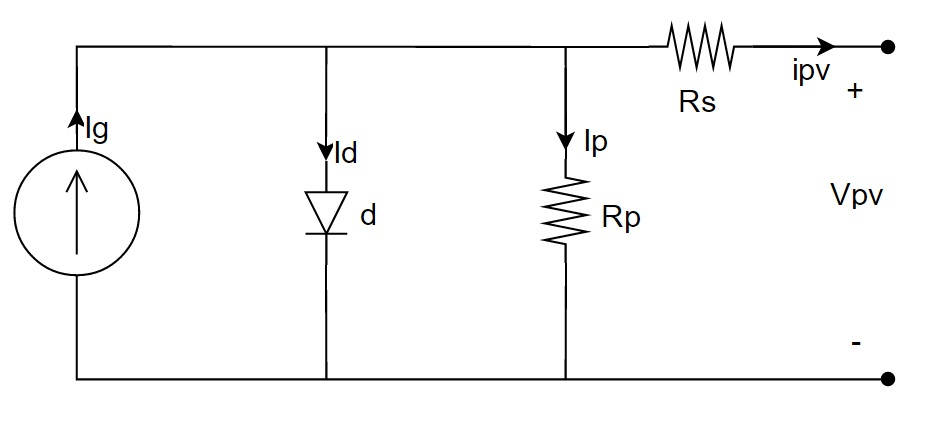
\includegraphics[scale=0.5]{./M2PV.jpg}
    \rule{35em}{0.5pt}
  \caption[Modelo con perdidas para un PV]{ Modelo con perdidas para un PV}
  \label{fig:Modelo2_PV}
\end{figure}

A partir del modelo con perdidas se puede deducir la ecuación que describe las corrientes, como sigue a continuación[4]:

\begin{equation} \label{eq:ej1}
  i_{pv}
  = I_{s} - i_{d} + i_{p}
\end{equation}

\begin{equation} \label{eq:ej2}
  I_{g}
  =
  2i_{pv} + \frac{V_{pv}+i_{pv}R_{s}}{R_p} -  I_{s} + I_{s}e^{ \frac{V_{pv}+i_{pv}V_{pv}}{n v_t}} 
\end{equation}

\textsl{Despejando $\ i_{pv}$}

\begin{equation} \label{eq:ej3}
  i_{pv} 
  =
  \frac{1}{2} \left[I_{s} + I_{g} - \frac{V_{pv}+i_{pv}R_{s}}{R_p} - I_{s}e^{ \frac{V_{pv}+i_{pv}V_{pv}}{n v_t}} \right]
\end{equation}
  
  
En general, la corriente que fluye por las terminales de un generador fotovoltaico está determinado por tres funciones de corriente:
\begin{compactitem}
\item \nt{Ig}: Corriente generada debido al efecto fotoeléctrico
\item \nt{id}: Corriente de pérdida debido a la juntura p-n
\item \nt{ip}: Corriente de pérdida de naturaleza resistiva
\end{compactitem}


 Para obtener un modelo del comportamiento estático del generador fotovoltaico se supondrá lo siguiente:

\begin{compactitem} 
\item \nt{Ig}: depende de la Irradiancia (S), pero no depende de la tensión en las terminales del generador fotovoltaico (\nt{Vpv})
\item \nt{ip} e \nt{id}: dependen de la tensión \nt{Vpv}
\item \nt{ip}: Depende de la temperatura (T)
\end{compactitem}

\textsl{De esta forma, la expresión que define $\ i_{pv}$}

\begin{equation} \label{eq:ej4}
  i_{pv} \left(V_{pv},T,S \right) 
  =
  i_g \left(V_{pv}\right)-i_d \left(V_{pv},T\right)
\end{equation}

\textsl{Según se definan las funciones $\ i_{pv}$ e $\ i_{d}$ se obtendrán modelos con complejidad y precisiones distintas, como los siguientes casos:  }


\begin{table}[H]
\centering
\caption{Modelos para un PV}
\label{Table:Modelos}
\begin{tabular}{|l|c|c|c|}
\hline
Modelos                                                             & $\ i_g$     & $\ i_p$ & $\ i_d$       \\ \hline
\begin{tabular}[c]{@{}c@{}} 1
\end{tabular}  & $\ KS $ & -   & $\ I_s\left(T\right)\left[e^\frac{V_{pv}}{v_t}-1\right] $          \\ \hline
\begin{tabular}[c]{@{}c@{}} 2
\end{tabular} & $\ KS $ & $\ G_pV_{pv} $   & $\ I_s\left(T\right)\left[e^\frac{V_{pv}}{v_t}-1\right] $          \\ \hline

\begin{tabular}[c]{@{}c@{}} 3 
\end{tabular} & $\ KS $ & -   & $\ I_s\left(T\right)\left[e^\frac{V_{pv} + i_{pv}R_{s} }{v_t}-1\right] $          \\ \hline
\begin{tabular}[c]{@{}l@{}} 4
\end{tabular} & $\ KS $ & $\ G_pV_{pv} + G_pi_{pv}R_s $   & $\ I_s\left(T\right)\left[e^\frac{V_{pv} + i_{pv}R_{s}}{v_t}-1\right] $     \\ \hline

\end{tabular}
\end{table}

De manera general se tiene: 

\begin{equation} \label{eq:ej5}
  i_{pv} \left(V_{pv}\right) 
  =
  G_{p}V_{pv} + G_{p}i_{pv}R_s
\end{equation}


\begin{equation} \label{eq:ej6}
  i_{d} \left(V_{pv}\right) 
  =
  I_s \left(T \right) e^\frac{V_{pv}}{v_t} e^\frac{ i_{pv}R_{s}}{v_t} -I_s \left(T \right)
\end{equation}

De esta forma el modelo general del comportamiento estático de un generador FV también se puede representar de la siguiente manera: 

\begin{equation} \label{eq:ej7}
  i_{pv}  
  =
  KS - G_{p}V_{pv} + I_s \left(T \right) - G_{p}i_{pv}R_s - I_s \left(T \right) e^\frac{V_{pv}}{v_t} e^\frac{ i_{pv}R_{s}}{v_t} 
\end{equation}

\begin{equation} \label{eq:ej8}
  I_s \left(T \right) e^\frac{V_{pv}}{v_t} e^\frac{ i_{pv}R_{s}}{v_t}   
  =
  KS - G_{p}V_{pv} + I_s \left(T \right) - G_{p}i_{pv}R_s - i_{pv} 
\end{equation}

La ecuación \ref{eq:ej8} es no lineal, aplicando una linealización, se tiene [3]: 

\begin{equation} \label{eq:ej9}
  y = ln \left(KS - G_{p}V_{pv} + I_s \left(T \right) - G_{p}i_{pv}R_s - i_{pv} \right) 
\end{equation}

si $ I_g = KS >> I_s $

\begin{equation} \label{eq:ej10}
  y = ln \left(KS - G_{p}V_{pv} - G_{p}i_{pv}R_s - i_{pv} \right) 
\end{equation}

\begin{equation} \label{eq:ej11}
  z = V_{pv} + i_{pv}R_s  
\end{equation}

posteriormente a un proceso de calculo de parámetros se tiene: 

\begin{equation} \label{eq:ej12}
  \theta_1  = ln\left( I_s \left(T \right) \right)
\end{equation}

\begin{equation} \label{eq:ej13}
  \theta_2  = \alpha 
\end{equation}

\section{Algoritmo de CORDIC}

El algoritmo \nt{Coordinate Rotational DIgital Computer} (CORDIC) es un método numérico en donde se realiza cierto numero de iteraciones para encontrar el valor deseado según sea la función en calculo, este algoritmo es utilizado para implementar funciones trigonométricas, logarítmicas y  exponenciales. La facilidad de implementación, hace que sea uno de los algoritmos mas utilizados en el ámbito de la electrónica digital, CORDIC utiliza desplazamientos, sumas, restas y tablas look-up con valores previamente precargados en una memoria ROM, estos valores dependerán de la operación en calculo, se puede utilizar el método circular, lineal e hiperbólico.   

Las ecuaciones generales para el algoritmo de CORDIC se definen como: 

\begin{equation} \label{eq:ej14}
  X_{i+1} = X_{i}- md_{i} 2^{-i} Y_{i}  
\end{equation}

\begin{equation} \label{eq:ej15}
  Y_{i+1} = Y_{i}- d_{i} 2^{-i} X_{i}  
\end{equation}

\begin{equation} \label{eq:ej16}
  Z_{i+1} = Z_{i}- d_{i} e\left(i\right)
\end{equation}

donde $\ e\left(i\right) $ se muestra en la tabla \ref{Table:ei} [5] según sea el caso:

\begin{table}[H]
\centering
\caption{Sistema de coordenadas unificado (CORDIC)}
\label{Table:ei}
\begin{tabular}{|l|c|c|c|}
\hline
m & Sistema de coordenadas                                                             & Valor de $\ e\left(i\right) $     \\ \hline
\begin{tabular}[c]{@{}c@{}} 1
\end{tabular}  & Circular & $\ tan^{-1}\left(2^{-i}\right)$         \\ \hline
\begin{tabular}[c]{@{}c@{}} 0
\end{tabular} & Lineal & $\ 2^{-1} $          \\ \hline

\begin{tabular}[c]{@{}c@{}} -1 
\end{tabular} & Hiperbólico & $\ tanh^{-1}\left(2^{-i}\right)$                \\ \hline


\end{tabular}
\end{table}



\subsection{Sistema de coordenadas hiperbólico}

Para el calculo de algunas funciones que no son tan directas con el algoritmo, se utilizan identidades [6] para el calculo como sigue:

\begin{equation} \label{eq:ej17}
  \tan z = \frac{\sin z}{\cos z}
\end{equation}

\begin{equation} \label{eq:ej18}
  \tanh z = \frac{\sinh z}{\cosh z}
\end{equation}

\begin{equation} \label{eq:ej19}
  \exp z = \sinh z + \cosh z
\end{equation}

\begin{equation} \label{eq:ej20}
  \ln \omega = 2 \tanh^{-1} \left( \frac{y}{x} \right)
\end{equation}

donde: 

\begin{equation} \label{eq:ej21}
  x = \omega + 1
\end{equation}

\begin{equation} \label{eq:ej22}
  y = \omega - 1
\end{equation}

\subsubsection{Logaritmo natural utilizando el algoritmo hiperbólico de CORDIC}
Para un $\ Ln \left(\omega\right) $  con el algoritmo de CORDIC, se debe calcular primeramente la $\ \tanh^{-1} \left( \frac{y}{x} \right)$ con las siguientes ecuaciones:

 
\begin{equation} \label{eq:ej23}
  X_{i+1} = X_{i} + d_{i} 2^{-i} Y_{i}  
\end{equation}

\begin{equation} \label{eq:ej24}
  Y_{i+1} = Y_{i} + d_{i} 2^{-i} X_{i}  
\end{equation}

\begin{equation} \label{eq:ej25}
  Z_{i+1} = Z_{i} - d_{i} tanh^{-1}\left(2^{-i}\right)
\end{equation}

donde $\ i $ es el indice de cada iteración, las iteraciones 4, 13, 40,… k, 3k+1 se deberán repetir para garantizar la convergencia. $\ d_i $ es el signo de $\ Y_i $ invertido, es decir el cuando el signo de $\ Y_i $ es negativo, $\ d_i $ será positivo y viceversa.

Utilizando la ecuación \ref{eq:ej20} se definen los valores de entrada para las ecuaciones anteriores  $\ X_0 = \omega + 1$ , $\ Y_0 = \omega - 1$ y $\ Z_0 = 0 $.

Cabe destacar que el rango de convergencia para este algoritmo [7] se puede definir como: 

\begin{equation} \label{eq:ej26}
   0.106843 \leq \omega \leq 9.35947
\end{equation}

donde $\ \omega $ es el valor del argumento del logaritmo natural.

El resultado final de $\ Z_i $ contiene el valor de $\ \tanh^{-1} \left( \frac{y}{x} \right)$, sin embargo se debe multiplicar por un factor de 2 para completar el calculo del logaritmo natural, segun la identidad de la ecuación \ref{eq:ej20} 

\subsubsection{Exponencial utilizando el algoritmo hiperbólico de CORDIC }


Para una función  $\ e^{\left(\omega\right)} $  con el algoritmo de CORDIC, se debe utilizar las ecuaciones \ref{eq:ej23}, \ref{eq:ej24} y \ref{eq:ej25} de manera iterativa, donde el valor final de $\ X $ y $\ Y$, son el resultado para  $\\cosh\left(\omega\right)$ y $\ \sinh\left(\omega\right)$ respectivamente. se debe tomar en cuenta la repeticion de las iteraciones $\ \left(i\right) $ 4, 13, 40,… k, 3k+1 para garantizar la convergencia dando una mejor precision en el calculo.

Los valores iniciales se definen como \nt{constantes} $\ X_0 = 1.20753406 $ , $\ Y_0 = 0$ y $\ Z_0 = \omega $ donde $\ \omega$  es el valor del argumento que se desea calcular y $\ d_i $ es el signo de $\ Z_i $.

Cabe destacar que el rango de convergencia para este algoritmo se puede definir como: 

\begin{equation} \label{eq:ej26}
   0 \leq \omega \leq 1
\end{equation}

El valor final del calculo se obtiene mediante una suma con la identidad de la ecuación \ref{eq:ej19}. 




\subsection{Referencias bibliográficas}

[1] Suskis, Pavels, and Ilya Galkin. "Enhanced photovoltaic panel model for MATLAB-simulink environment considering solar cell junction capacitance." Industrial Electronics Society, IECON 2013-39th Annual Conference of the IEEE. IEEE, 2013.

[2] González-Longatt, Francisco M. "Model of photovoltaic module in Matlab." II CIBELEC 2005 (2005): 1-5.

[3] C. Meza, R. Ortega, "Control and estimation scheme for PV central inventers", in 24th International Conference on information, Comunication and Automation Technologies, Nov, 2013 

[4] Chiang, Ching-Tsan, Tung-Sheng Chiang, and Hou-Sheng Huang. "Modeling a photovoltaic power system by CMAC-GBF." Photovoltaic Energy Conversion, 2003. Proceedings of 3rd World Conference on. Vol. 3. IEEE, 2003.

[5] Ibrahim, Muhammad Nasir, et al. "Hardware Implementation of Math Module Based on CORDIC Algorithm Using FPGA." Parallel and Distributed Systems (ICPADS), 2013 International Conference on. IEEE, 2013.

[6] Walther, John S. "A unified algorithm for elementary functions." Proceedings of the May 18-20, 1971, spring joint computer conference. ACM, 1971.

[7] Llamocca-Obregón, Daniel R., and Carla P. Agurto-Ríos. "A fixed-point implementation of the expanded hyperbolic CORDIC algorithm." Latin American applied research 37.1 (2007): 83-91.










\index{referencias}\index{BibTeX}
Todo concepto o idea tomado de otros autores contar con la respectiva
referencia. En redacción técnica de ingeniería rara vez se utiliza la cita
textual, así que es necesario reformular las ideas y conceptos con palabras
propias. En ingeniería electrónica se utilizan los formatos de referencia de la
IEEE o la ACM, que son numéricos, encerrados entre paréntesis cuadrados (por
ejemplo, ``En \cite{Davis1963} se propuso un nuevo algoritmo'', o ``En
\cite{ProakisManolakis1998} los autores proponen tomar las ventajas de los
algorimos presentados en \cite{Oppenheim1998,Roberts2005,Haykin2001} por medio
del método de Newton \cite{Burrus1998} conocido en el área de optimización
lineal.''). La referencia es parte de las frases, así que si la frase termina
con la referencia para indicar la idea, ésta debe estar antes del punto final o
demás signos de puntuación: ``La capacidad de memoria también sigue una Ley
similar a la de Moore \cite{Octave}. Los siguientes son los aspectos a tomar en
cuenta en el diseño del sistema \cite{Lindner2002}:''

Se recomienda utilizar BibTeX para administrar las referencias bibliográficas.

\subsection{Extensión}

\index{extensión}
Una tesis de licenciatura no debe sobrepasar las 120 páginas incluyendo
apéndices y los formalismos desde portada hasta índices.

El cuerpo de la tesis (desde introducción hasta conclusiones) usualmente se
extiende desde 45 páginas hasta no más de 80, dependiendo de la problemática
tratada.

No es necesario reproducir contenidos de otras fuentes: agregue las referencias
a dichas fuentes, y limítese a enunciar lo estrictamente necesario para
comprender sus propuestas de solución.

\section{Sobre esta plantilla \LaTeX}

Esta plantilla \LaTeX pretende simplificar varios pasos en la creación del
documento de tesis.

\subsection{Marcar asuntos pendientes}

La plantilla tiene dos ``\emph{modos}'' de operación: normal y borrador
(\emph{draft}).  En el archivo \texttt{main.tex} a partir de la línea 41 usted
encuentra el código

\begin{verbatim}
%
% DRAFT MODE
%
\newboolean{draftmode}                  % boolean used to control draft-mode
% Ensure that only one of the next two lines is active:
\setboolean{draftmode}{true}            % turn draft mode on
%\setboolean{draftmode}{false}           % turn draft mode off
\end{verbatim}

Con el modo borrador, se activan ciertos comandos y funcionalidades útiles en
el proceso de elaboración de la tesis, pero que deben ser desactivados al
final, antes de entregar la tesis.  Por ejemplo, se activa el pie de página que
dice ``\emph{Borrador: fecha}'', y se activa el índice titulado ``Revisar''.  En dicho índice aparecen las páginas en donde se hayan utilizado alguno de los siguientes comandos:
\begin{compactitem}
\item \verb+\boxcomment{comentario}+ Crea una caja en el margen de página con
  el comentario indicado.
\item \verb+\explain{comentario}+ Crea una caja en el margen de página con
  el comentario indicado, con una flecha hacia la derecha para indicar qué en
  concreto debe ser revisado.
\item \verb+\chk{comentario}+ Crea una caja en el margen con símbolo de
  ``chequeado'' y el comentario indicado.
\item \verb+\TODO{comentario}+ Crea una caja grande de fondo sombreado con el
  comentario indicado.
\end{compactitem}

En este párrafo se\chk{resultado de chk} utilizan algunos de estos comandos
para ilustrar su efecto.  El \verb+\chk+ como puede observar tiene sentido
usarlo para marcar que algo está casi listo.  Por otro lado \explain{explain}
el comando \verb+\explain+ permite marcar algo que requiere ser revisado en
redacción, valores, etc.  El \verb+\boxcomment+\boxcomment{La caja simple}
solo pone una marca al margen.

\TODO{Finalmente el comando \texttt{TODO} coloca esta caja gris.}

Si usted desativa el modo draft, desaparecen todas las páginas, y desaparece el
índice ``Revisar''.  En éste índice aparecen todas las páginas en donde se
utilizaron estos comandos con los respectivos comentarios, lo que permite
encontrar rápidamente detalles que usted indicó que debe revisar.

\subsection{Índices}

Como índice se conoce la lista de términos claves con su respectiva página, al
final del documento.  La plantilla ofrece varios comandos para simplificar el
uso estandar del comando de \LaTeX\ \verb+\index{termino}+ que coloca al término
indicado en el índice.  Con \verb+\nt[indice]{termino}+ (\emph{new term}) usted
indica la entrada principal del término, que aparece en el texto en el índice,
es decir, en el índice aparece lo que indique en vez de ``indice'' y en el
texto aparece lo que indique ``termino''; \verb+\ot{termino}+ agrega una
entrada secundaria al término.

  \chapter{Sistema de linealización}
\label{ch:linealizacion}

Para realizar la linealización de la expresión exponencial de la corriente $\ i_{pv} $ del modelo del panel, se implementa una función logarítmica, dentro de los algoritmos de cálculo se tiene el de CORDIC, este permite realizar una aproximación de la función de manera recursiva mediante cierta cantidad de iteraciones, para el caso del linealizador se utiliza el método hiperbólico para realizar el cálculo de la operación logaritmo natural, este algoritmo requiere de una tabla (Look-up table) con valores pre-cargados. 

El rango de convergencia para este algoritmo es de $\ 0.106843 < T < 9.35947 $ donde $\ T $ es el argumento del logaritmo natural, el valor máximo de $\ T $ para el panel previamente escogido de 0.58A, esta es la corriente en condiciones máximas para el panel, debido a esto se puede desplazar el intervalo que se tiene para los argumentos de la función, este se divide entre una constante $\ C = 16$ y se desplaza $\ 0.00667769 < T < 0.58496687 $, esto se realizó debido a que se pueden dar valores de corriente mas bajos que 0.106843A. Esta constante C se debe compensar en el logaritmo, y se logra con la siguiente igualdad: 

\begin{equation} \label{eq:ej1}
  Ln \left( T \right)
  = Ln \left( 16T \right) - Ln\left( 16 \right) 
\end{equation}  

  

\section{Algoritmo de CORDIC en software}
 
Para comprobar el debido funcionamiento del este algoritmo se crea un programa de alto nivel en Python.  


\begin{figure}[H]
  \centering
    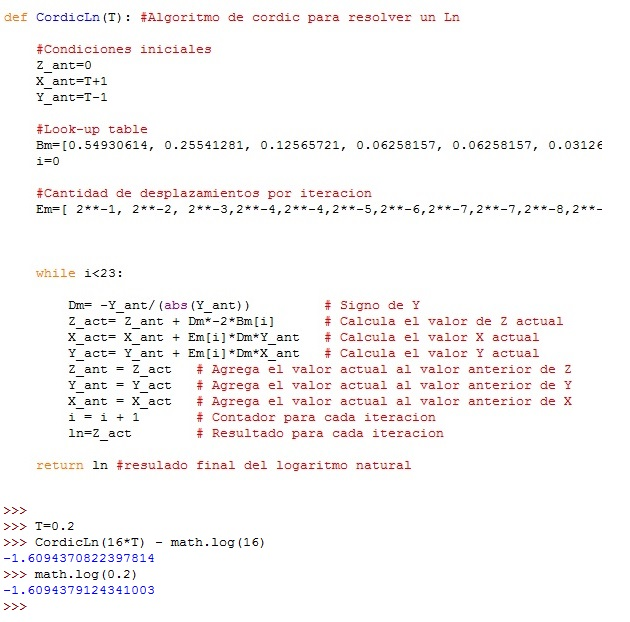
\includegraphics[scale=0.6]{./Progra_Cordic.jpg}
    \rule{35em}{0.5pt}
  \caption[Algoritmo de CORDIC en Python]{Algoritmo de CORDIC en Python  }
  \label{fig:Python}
\end{figure}


En la figura \ref{fig:Python} se observa el programa realizado para la verificación del algoritmo, para este se utilizan las ecuaciones del marco teórico descritas con anterioridad, también se comprueba el cambio en el rango de cálculo con el escalado del argumento por 16. 

Para simplificar el diseño del hardware se realizan cambios en las ecuaciones originales, se cambia la resta del valor actual de Z por una suma, y se incluye el signo en la LUT de Z, el resultado final del algoritmo se debe multiplicar por 2, sin embargo este escalado se puede realizar en la LUT, esto para evitar la multiplicación, esto se comprueba en el programa de la figura \ref{fig:Python}.  


\section{Sistema linealizador con el algoritmo de CORDIC}

\begin{figure}[H]
  \centering
    \includegraphics[scale=0.06]{./Linealizador_general.png}
    \rule{35em}{0.5pt}
  \caption[Bloque principal: algoritmo de CORDIC en hardware]{Bloque principal: Algoritmo de CORDIC en hardware  }
  \label{fig:CORDIC1}
\end{figure}

La figura \ref{fig:CORDIC1} contiene el bloque general del algoritmo de CORDIC, poseen 4 entradas: CLK , T , Begin\_LN , RST\_LN y 4 salidas: ACK\_LN , RESULT , U\_F , O\_F

\begin{figure}[H]
  \centering
    \includegraphics[scale=0.05]{./Linealizador_CORDIC_FSM.png}
    \rule{35em}{0.5pt}
  \caption[Coprocesador CORDIC y Control]{Coprocesador CORDIC y Control  }
  \label{fig:CORDIC2}
\end{figure}

El sistema de linealización de la figura \ref{fig:CORDIC2} cuenta con dos módulos principales: 

\begin{compactitem}

\item \nt{Coprocesador Cordic}: En este realizan todas las operaciones requeridas por el algoritmo, se encarga del manejo de los datos en el cálculo. 


\item \nt{Control}: Este se encarga de proveer las señales de control requeridas por el coprocesador, según las condiciones que se tenga en cada estado.

\end{compactitem}

Señales de datos: 

\begin{compactitem}

\item \nt{T}: Dato de entrada, argumento del logaritmo natural. 
\item \nt{RESULT}: Resultado de la operación logaritmo natural.

\end{compactitem}

Señales de control: 

\begin{compactitem}
\item \nt{CLK}: Reloj del sistema. 

\item \nt{Begin\_LN}: Esta se encarga de dar inicio a la operación logaritmo natural. 

\item \nt{RST\_LN}: Realiza un reset a la unidad CORDIC tanto para el coprocesador como para la máquina de estados.
 

\item \nt{ACK\_LN}: Indica que el cálculo ya fue realizado.

\item \nt{Begin\_SUM}: Esta se encarga de dar inicio a la unidad de suma-resta punto flotante.

\item \nt{ACK\_SUM}: Indica que esta listo el calculo realizado en la unidad de suma-resta punto flotante.

\item \nt{O\_F}: Indica si la suma-resta flotante realizada tiene un over-flow.

\item \nt{U\_F}: Indica si la suma-resta flotante realizada tiene un under-flow.

\item \nt{CLK\_DIR}: Activa el enable del contador de iteraciones. 

\item \nt{CONT\_ITER}: Indica el numero de iteración, para que la máquina de estados pueda detenerse en el número que se le asigne.
 
\item \nt{RST}: Realiza el reset de todos los registros de la unidad.

\item \nt{MS\_1 , MS\_2 , MS\_3 , MS\_4}: Realizan la selección de cada multiplexor, Mux1, Mux2, Mux3, Mux's4 respectivamente.

\item \nt{EN\_REG1X , EN\_REG1Y , EN\_REG1Z}: Activa los enable de los registros de la primera etapa REG1X, REG1Y, REG1Z respectivamente, para almacenar datos. 

\item \nt{EN\_REG2XYZ}: Activa el enable del registro REG2XYZ de la segunda etapa. 

\item \nt{EN\_REG2}: Activa el enable del registro REG2 de la segunda etapa.

\item \nt{EN\_REG3}: Activa el enable del registro REG3 del dato inicial.

\item \nt{EN\_REG4}: Activa el enable del registro REG4 del dato final. 

\end{compactitem}

\section{Coprocesador CORDIC}
El diseño de este algoritmo se basa en una arquitectura segmentada, de manera que se almacenan y procesan varios datos a la vez, sin embargo se debe tener buena sincronización para evitar datos erróneos a través del proceso de cálculo. Por otro lado se utiliza el formato IEEE 754 con 32Bits, esto debido a que se requiere una adecuada precisión en el calculo y un menor número de iteraciones, repercutiendo en la velocidad del sistema. 

\begin{figure}[H]
  \centering
    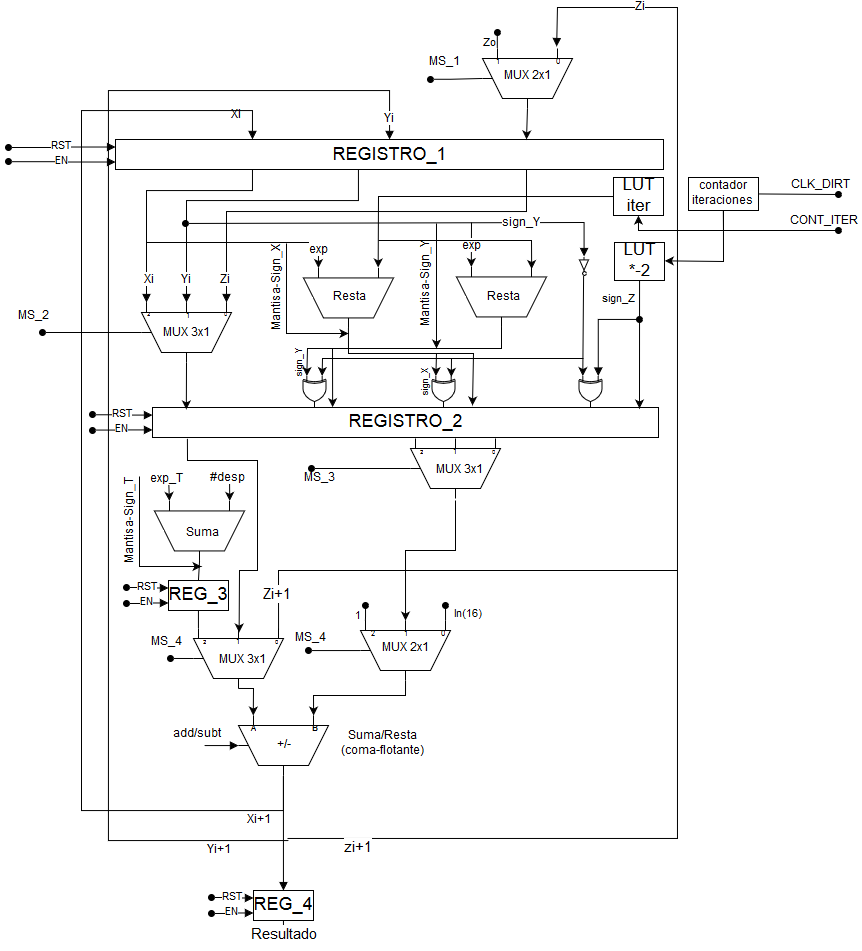
\includegraphics[scale=0.04]{./CORDICLN.png}
    \rule{35em}{0.5pt}
  \caption[Coprocesador segmentado para el cálculo de una función logarítmica con el algoritmo de CORDIC en hardware]{Coprocesador segmentado para el cálculo de una función logarítmica con el algoritmo de CORDIC en hardware  }
  \label{fig:CORDICLN}
\end{figure}

En la figura \ref{fig:CORDICLN} se puede observar la arquitectura diseñada para el algoritmo de CORDIC, con el formato IEEE 754 en 32-Bits, se trabaja en punto flotante, este reduce el numero de iteraciones, y produce una mejor precisión tanto en las operaciones como el resultado final. 

Esta etapa inicia con la carga de las condiciones iniciales, donde $\ Z_0 $ contiene un valor inicial cero, para el valor inicial de $\ X_0 $ y $\ Y_0 $ primeramente se aplica el escalado  16*T,
este escalado se puede representar como un desplazamiento $\ 2^{-4} $, por lo tanto este movimiento en punto flotante se traduce como una suma de 4 en el exponente de $\ T$, posteriormente se realizan las siguientes operaciones en punto flotante,  $\ X_0 = T + 1 $ y $\ Y_0 = T - 1 $, estas tres constantes dan inicio al proceso de cálculo de manera iterativa, por lo que se requiere almacenarlas en un registro en la primera etapa de segmentación $\ \left(Registro 1 \right) $, los nuevos estados se deben calcular uno por uno, esto debido a que el circuito para el sumador-restador en punto flotante requiere de mucha área, este método (CORDIC) es un calculo cruzado es decir, para el próximo valor de $\ X_i$ se requiere un valor de $\ Y_0 $ con un desplazamiento y un cambio de signo, y para $\ Y_i $ se aplica un concepto similar con valores de $\ X_0$,  por lo tanto para el cálculo de $\ X_i $ se requiere un restador en punto fijo para desplazar el valor del exponente de $\ Y_0 $ , para el nuevo valor de $\ Y_i $ se utiliza un restador punto fijo para el valor del exponente de $\ X_0 $ y para $\ Z_i $ se requiere una ROM con valores previamente cargados $\ \left(LUT \right) $. Estas operaciones "$\ X_i , Y_i $"  involucran el signo de "$\ Y_0 $" invertido.

Para el signo de las operaciones CORDIC se utiliza un circuito de comparación como se observa en la siguiente tabla: 

\begin{table}[H]
\centering
\caption{Tabla de signo $\ \delta $ para cada iteración componente Xi , Yi , Zi}
\label{Table:Signo}
\begin{tabular}{|c|c|c|c|c|c|c|}
\hline
Sign $\ X_0 $ & Sign $\ Z_0 $  & Sign $\ Y_0 $ & Sign $\ \sim Y_0 $  & Sign $\ X_i $ & Sign $\ Z_i $  & Sign $\ Y_i $      \\ \hline

\begin{tabular}[c]{@{}c@{}} 0
\end{tabular}  & 0 & 0   & 1   & 1 & 1 & 1       \\ \hline

\begin{tabular}[c]{@{}c@{}} 0
\end{tabular} & 0 & 1   & 0  & 0 & 0 & 1       \\ \hline

\begin{tabular}[c]{@{}c@{}} 0 
\end{tabular} & 1 & 0   & 1 & 1 & 0 & 1\\ \hline
\begin{tabular}[c]{@{}l@{}} 0
\end{tabular} & 1 & 1   & 0  & 0 & 1 & 1   \\ \hline

\begin{tabular}[c]{@{}l@{}} 1
\end{tabular} & 0 & 0   & 1 & 0 & 1 & 1   \\ \hline

\begin{tabular}[c]{@{}l@{}} 1
\end{tabular} & 0 & 1   & 0  & 1 & 0 & 1   \\ \hline

\begin{tabular}[c]{@{}l@{}} 1
\end{tabular} & 1 & 0   & 1  & 0 & 0 & 1   \\ \hline

\begin{tabular}[c]{@{}l@{}} 1
\end{tabular} & 1 & 1   & 0 & 1 &  1 & 1    \\ \hline


\end{tabular}
\end{table}

\begin{figure}[H]
  \centering
    \includegraphics[scale=0.06]{./signo.png}
    \rule{35em}{0.5pt}
  \caption[Signo $\ \delta$ para cada iteración componente Xi , Yi , Zi]{Signo $\ \delta$ para cada iteración componente Xi , Yi , Zi   }
  \label{fig:SGN}
\end{figure}


A partir de la tabla \ref{Table:Signo} se extrae el circuito de comparación de signo de la figura \ref{fig:SGN}, este es diseñado con compuerta \nt{XOR} que poseen el mismo comportamiento de la tabla. 


Se requiere de dos Look-up tables "LUT", los datos de cada tabla se almacenan en memorias ROM's, de manera que puedan ser accesados en cualquier momento que sean requeridos por medio de la dirección, dentro de las ROM's se dispone:   

\begin{compactitem}

\item \nt{LUT\_Z}: Contiene almacenados los valores de $\ -2arctanh \left( 2^{-i} \right) $, para cada iteración.  
\item \nt{LUT\_ITER}: Esta contiene almacenados los desplazamientos que se deben realizar para cada iteración, esto debido a que las iteraciones 4 y 13 repiten desplazamientos como se menciona en el marco teórico. 

\end{compactitem}

El acceso a cada valor de la tablas se realiza mediante un contador de iteraciones, este indica a cada tabla la dirección que debe desplegar según el numero de iteración.  

El proceso para el cálculo de las variables no se puede realizar de manera simultanea, ya que solo se cuenta con un sumador punto flotante, para esto se cuenta con las variables iniciales del registro 1 y se almacenan las variables modificadas en el \nt{Registro 2}, la secuencia de cálculo toma primeramente los valores que se necesitan para  $\ X_i $, posteriormente se realiza el cálculo y se almacena el resultado en el \nt{Registro 1}, seguidamente se procede con el cálculo de $\ Y_i $ y se almacena en el \nt{Registro 1}, por ultimo se calcula el valor de $\ Z_i $, concluida la suma se almacena en el \nt{Registro 1}, este proceso se hace de manera iterativa, una vez finalizada la cuenta de N iteraciones según se defina (N=numero entero), se realiza la resta $\ Z_i - Ln\left(16\right) $ para contrarrestar el efecto del escalado aplicado al argumento $\ \left(T\right) $ al inicio del cálculo del logaritmo natural, por último el resultado final de $\ Z_i $ contiene el valor de $Ln \left(T \right)$ , este se almacena en el \nt{Registro 4}.

\section{Sistema de control para el coprocesador CORDIC (FSM)}

\begin{figure}[H]
  \centering
    \includegraphics[scale=0.045]{./MaquinaL.png}
    \rule{35em}{0.5pt}
  \caption[Maquina de estados finitos para la arquitectura de CORDIC]{Maquina de estados finitos para la arquitectura de CORDIC   }
  \label{fig:FSML}
\end{figure}

El sistema de control requiere de mucha sincronía, ya que los datos debe ser almacenados de manera correcta y estar listos cuando se requiere por otro segmento del coprocesador CORDIC, para esto se diseñó una maquina de estados finitos, donde inicialmente se calculan los valores iniciales de $ X_0 $, $ Y_0 $ y $ Z_0 $, posteriormente la maquina brinda las señales de control requeridas con la secuencia de cálculo de $ X_i $,$ Y_i $ y $ Z_i $ respectivamente realizando una cuenta de iteración, se cuenta con una variable de entrada para que este control pueda saber el número de iteración en el que se encuentra, de manera que cuando se llega a la iteración N definida con anterioridad, se finaliza el cálculo.

\section{Algoritmo de CORDIC en Verilog}

Este algoritmo se implementó por medio de el lenguaje de descripción de hardware "Verilog", inicialmente se realizaron pequeños bloques pertenecientes a cada elemento requerido por la arquitectura diseñada, se vio la necesidad, por cuestión de orden, de desarrollar el coprocesador CORDIC y la unidad de control en bloques separados, de manera que se pudieran realizar pruebas sin dependencia de los bloques entre si, para una mejor depuración de errores y re-diseño. Finalmente se realizan las simulaciones al bloque completo en la figura \ref{fig:SIMLINEAL}. 

\begin{figure}[H]
  \centering
    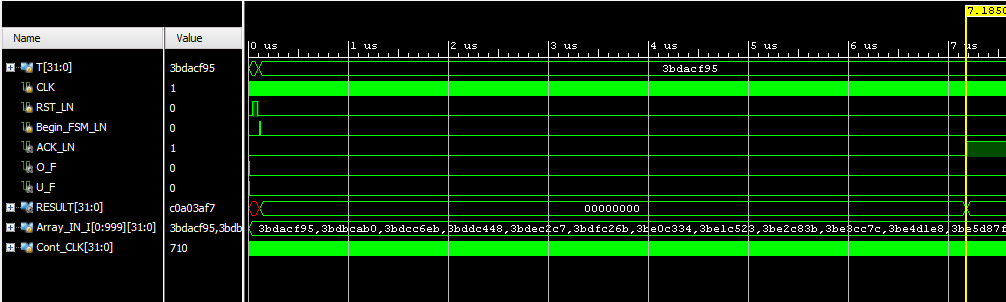
\includegraphics[scale=0.6]{./TEST_LINEALIZADOR_I.png}
    \rule{35em}{0.5pt}
  \caption[Simulación del linealizador en implementado en Verilog]{Simulación del linealizador en implementado en Verilog}
  \label{fig:SIMLINEAL}
\end{figure}   

\section{Simulación del circuito linealizador con algoritmo de CORDIC}

Las simulaciones de la implementación del algoritmo, se realizaron mediante mil valores de entrada, obteniendo así mil valores de salida, los cuales se comparan con los valores reales, para dicha comparación se realizaron aproximaciones con 8, 12 y 15 iteraciones. 

Primeramente se realiza una simulación que comprueba el funcionamiento en el rango de operación $\ 0.00667769 < T < 0.58496687 $ y la linealización esta prueba se realiza con la siguiente función: 

\begin{equation} \label{eq:ej2}
  Ln \left(T \right) 
\end{equation} 

donde el argumento T es:

\begin{equation} \label{eq:ej3}
   T = e^{-x}         
\end{equation} 
  
El intervalo $\ 0,536 < x < 5,009$ se divide en mil valores, de manera que la función \ref{eq:ej2} devuelve mil valores, estos se almacenan en un archivo .txt de manera que se insertan en el circuito CORDIC para obtener mil valores del cálculo. 


\begin{equation} \label{eq:ej4}
   V_{pv} = V_{cte} + 0.3*V_{cte}*sin(2* \pi *100*t)     
\end{equation}


    
\begin{equation} \label{eq:ej5}
   i_{pv} = Ig - \frac{V_{pv}}{R_p} - Is*\left(e^\frac{V_{pv}* \alpha}{2}\right)         
\end{equation} 


Seguidamente se realiza una prueba con mil valores simulando el comportamiento que tiene un PV, utilizando el modelo del panel, donde se utiliza el valor de $ V_{pv} $ para cada valor de tiempo, en la ecuación \ref{eq:ej5} obteniendo valores de corriente de entrada $ i_{pv} $ para el linealizador, así poder observar si se realiza la linealización en la salida. 



\subsection{Resultados de la simulación del rango de convergencia del circuito linealizador CORDIC}

En la implementación de un algoritmo en hardware, es de suma importancia verificar que este funcione de manera adecuada en el rango de convergencia definido. Para la comprobación del algoritmo de la unidad del linealizador CORDIC, se realizaron una serie de pruebas, simulando con cierta cantidad de iteraciones y así poder observar cual es la mas adecuada para el cálculo requerido y su debido resultado, para esto se programó un simulación("testbench") en donde se corre una prueba con mil valores de entrada, ingresados por medio de un archivo de texto previamente editado con los datos de entrada con la función exponencial anteriormente descrita en la ecuación \ref{eq:ej3}. 


\begin{figure}[H]
  \centering
    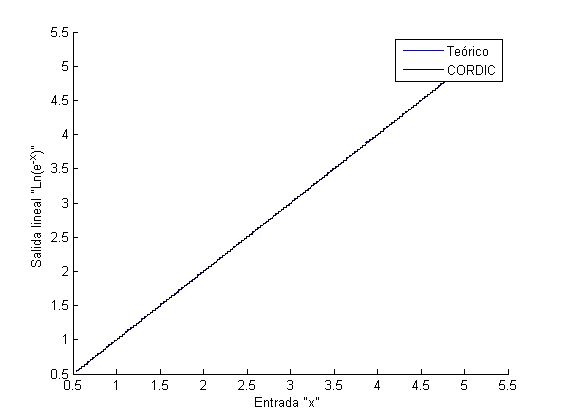
\includegraphics[scale=0.7]{./RANGO_8iter.png}
    \rule{35em}{0.5pt}
  \caption[Datos de la simulación post-sintesis del linealizador para un rango de convergencia CORDIC con 8 iteraciones]{Datos de la simulación post-sintesis del linealizador para un rango de convergencia CORDIC con 8 iteraciones  }
  \label{fig:RG8}
\end{figure}

\begin{figure}[H]
  \centering
    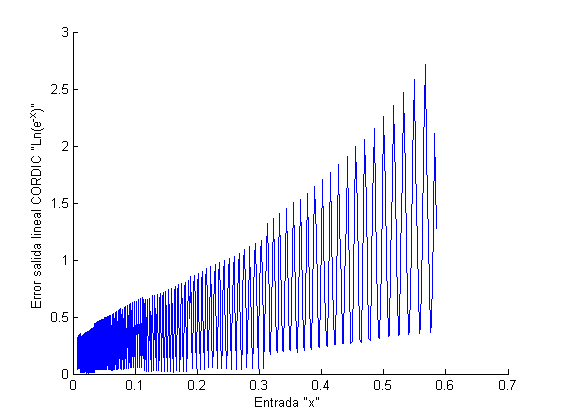
\includegraphics[scale=0.7]{./RANGO_8iter_ERROR.png}
    \rule{35em}{0.5pt}
  \caption[Porcentaje de error rango de convergencia circuito CORDIC con 8 iteraciones simulación post-síntesis]{Porcentaje de error rango de convergencia circuito CORDIC con 8 iteraciones simulación post-síntesis}
  \label{fig:RGE8}
\end{figure}


Primeramente se realizó una simulación con 8 iteraciones, como se muestra en la figura \ref{fig:RG8}, para el cálculo de cada valor se requieren 460 ciclos de reloj desde el momento en se activa la señal Begin\_LN hasta que se recibe la señal ACK\_LN, que es donde se indica que se ha completado el cálculo, es de suma importancia realizar la comparación entre el valor teórico y el valor calculado obtenido. Para cada valor se calculó el error, estos se pueden observar en la figura \ref{fig:RGE8}, donde el porcentaje de error máximo es de 2,72\% y el porcentaje de error promedio es de 0,40\%. 
 




\begin{figure}[H]
  \centering
    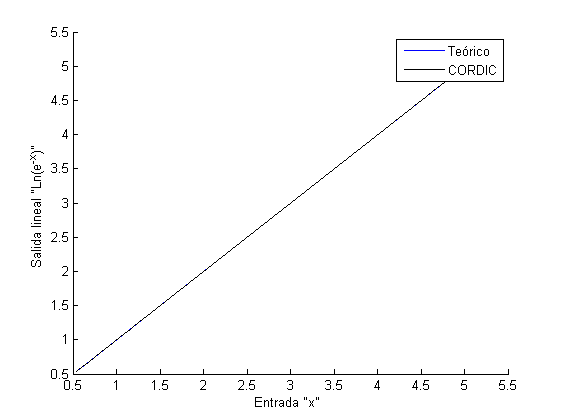
\includegraphics[scale=0.7]{./RANGO_12iter.png}
    \rule{35em}{0.5pt}
  \caption[Datos de la simulacion post-síntesis del linealizador para un rango de convergencia CORDIC con 12 iteraciones]{Datos de la simulación post-síntesis del linealizador para un rango de convergencia CORDIC con 12 iteraciones}
  \label{fig:RG12}
\end{figure}

\begin{figure}[H]
  \centering
    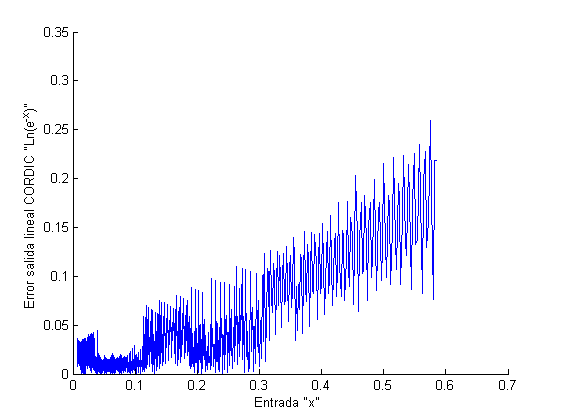
\includegraphics[scale=0.7]{./RANGO_12iter_ERROR.png}
    \rule{35em}{0.5pt}
  \caption[Porcentaje de error rango de convergencia circuito CORDIC con 12 iteraciones simulación post-síntesis]{Porcentaje de error rango de convergencia circuito CORDIC con 12 iteraciones simulación post-síntesis}
  \label{fig:RGE12}
\end{figure}

Una mejor aproximación se puede lograr utilizando 12 iteraciones en el calculo del logaritmo natural, en la figura \ref{fig:RG12} se pueden observar los resultados obtenidos, se requieren 660 ciclos de reloj para ejecutar el cálculo completo. La figura \ref{fig:RGE12} muestra el error en cada cálculo, donde el porcentaje de error máximo es de  0,259\% y el porcentaje de error promedio es de 0,0351\%. 

\begin{figure}[H]
  \centering
    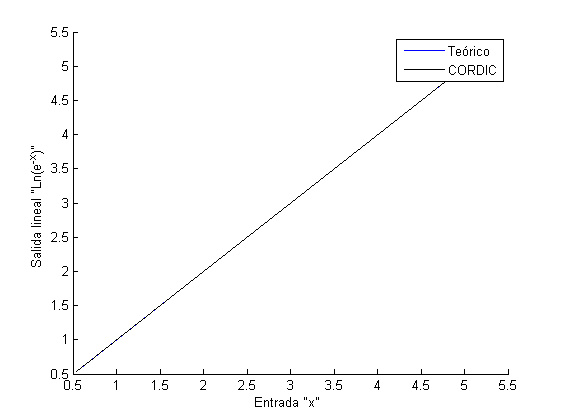
\includegraphics[scale=0.7]{./RANGO_15iter.png}
    \rule{35em}{0.5pt}
  \caption[Datos de la simulación post-síntesis del linealizador para un rango de convergencia CORDIC con 15 iteraciones]{Datos de la simulación post-síntesis del linealizador para un rango de convergencia CORDIC con 15 iteraciones}
  \label{fig:RG15}
\end{figure}

\begin{figure}[H]
  \centering
    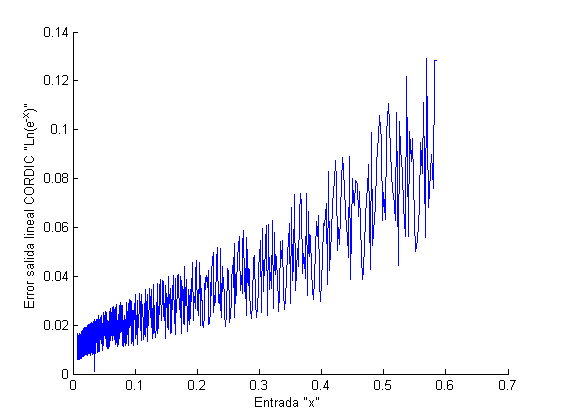
\includegraphics[scale=0.7]{./RANGO_15iter_ERROR.png}
    \rule{35em}{0.5pt}
  \caption[Porcentaje de error rango de convergencia circuito CORDIC con 15 iteraciones simulación post-síntesis]{Porcentaje de error rango de convergencia circuito CORDIC con 15 iteraciones simulación post-síntesis}
  \label{fig:RGE15}
\end{figure}


Utilizando 15 iteraciones en el cálculo del logaritmo natural se logra la mayor aproximación, sin embargo se requieren 818 ciclos de reloj y se vuelve mas lento el proceso, en la figura \ref{fig:RG15} se pueden observar los resultados obtenidos. La figura \ref{fig:RGE15} muestra el error en cada cálculo, donde el porcentaje de error máximo es de  0,129\% y el porcentaje de error promedio es de 0,0257\%. 


En las figuras de error \ref{fig:RGE8}, \ref{fig:RGE12} y \ref{fig:RGE15} se puede observar que el comportamiento del algoritmo es mas exacto cuando los valores de corriente de entrada del argumento de linealizador "T" son pequeños, a medida que este argumento se vuelve mayor el porcentaje de error también incrementa. 
  \chapter{Sistema de normalización}
\label{ch:Normalizacion}

El circuito realizado para la linealización se basa en el formato IEEE 754, sin embargo el estimador de parámetros que se tiene, esta basado en un formato punto fijo, de manera que se debe considerar una conversión entre ambos formatos, para esto se estudió como pasar de punto flotante a punto fijo, ambos en 32-bits.


\section{Sistema de conversión y normalización }

\begin{figure}[H]
  \centering
    \includegraphics[scale=0.6]{./FF_normalizador.png}
    \rule{35em}{0.5pt}
  \caption[Bloque general del convertidor puto flotante a punto fijo y normalizador]{Bloque general del convertidor puto flotante a punto fijo y normalizador. }
  \label{fig:FF-NORM}
\end{figure}


La figura \ref{fig:FF-NORM} contiene el bloque general del sistema de conversión y normalización , este posee 4 entradas: CLK , F , Begin\_FF , RST\_FF y 2 salidas: ACK\_FF , RESULT.

\begin{figure}[H]
  \centering
    \includegraphics[scale=0.6]{./FMS_FF_NORMALIZADOR.png}
    \rule{35em}{0.5pt}
  \caption[Sistema de convesión, normalización, señales de datos y control]{Sistema de conversión, normalización, señales de datos y control.}
  \label{fig:FMS_FF_NORM}
\end{figure}

El sistema de conversión y normalización de la figura \ref{fig:FMS_FF_NORM} cuenta con dos módulos principales: 

\begin{compactitem}

\item \nt{Convertidor-Normalizador}: En este realizan todas las operaciones requeridas para la conversión del formato Punto flotante- Punto fijo y de la normalización, este se encarga del manejo de los datos en el cálculo. 


\item \nt{Control}: Este se encarga de proveer las señales de control requeridas por el Convertidor-Normalizador, según las condiciones que se tenga y se requiera en cada estado.

\end{compactitem}

señales de datos: 

\begin{compactitem}

\item \nt{F}: Dato de entrada, este posee un valor en formato IEEE 754.
\item \nt{RESULT}: Dato de salida convertido de punto flotante a punto fijo.

\end{compactitem}

señales de control: 

\begin{compactitem}

\item \nt{CLK}: Reloj del sistema, este ejecuta ciclos de reloj con una frecuencia preestablecida. 

\item \nt{Begin\_FF}: Este se encarga de iniciar la la unidad, indica a la maquina de estados que inicia la secuencia. 

\item \nt{RST\_FF}: Este se encarga reestablecer los valores iniciales del sistema de conversión y normalización.

\item \nt{ACK\_FF}: Indica cuando la conversión y la normalización han sido realizadas.

\end{compactitem}


 

\section{Convertidor punto flotante - punto fijo y normalizador }


\begin{figure}[H]
  \centering
    \includegraphics[scale=0.5]{./conversion_FF.png}
    \rule{35em}{0.5pt}
  \caption[conversión y normalización]{Proceso de conversión y normalización  }
  \label{fig:FF}
\end{figure}



  En la figura \ref{fig:FF} se puede observar el diagrama de solución que se utilizó para el desarrollo del convertidor-normalizador , primeramente ingresa el numero en formato IEEE 754 32-bits, posteriormente se efectúa la conversión a punto fijo, en donde se asigna un bit de signo, 5 bits de parte entera y 26 bits para la parte fraccionaria, este dato se procesa en una etapa de normalización y se obtiene el resultado, este valor final esta normalizado para la corriente y tension del panel, $\ V = [0,1]$ e $\ i = [-1,1]$, para el formato punto fijo solo se requiere, un bit de signo, un bit en la parte entera y 30 para la parte fraccionaria, como se muestra en la figura \ref{fig:FF}, el aumento de bits en la parte fraccionaria indica una mejor precisión en el resultado. 

  
  \begin{figure}[H]
  \centering
    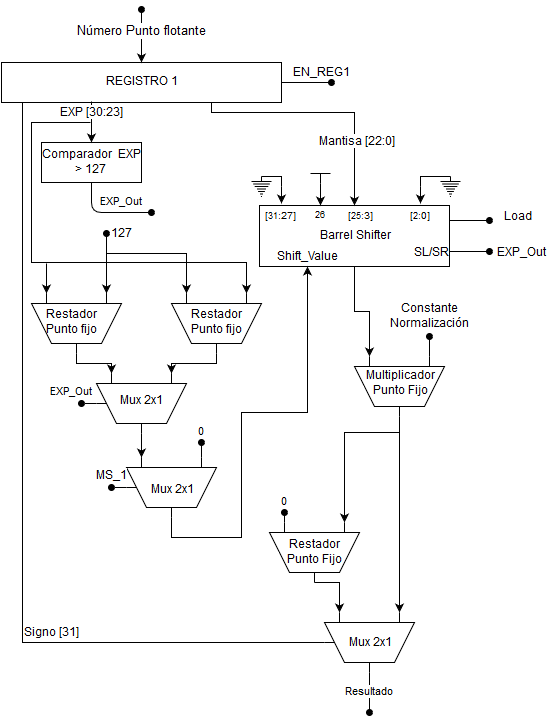
\includegraphics[scale=0.7]{./NORMALIZADOR.png}
    \rule{35em}{0.5pt}
  \caption[Normalizador]{Conversión punto flotante a punto fijo y normalización  }
  \label{fig:NORM}
\end{figure} 

Como se observa en la figura \ref{fig:NORM}, la etapa de conversión de formatos contiene un comparador, este se utiliza para saber si el numero en formato IEEE 754, contiene un exponente mayor o menor que 127, si el numero es igual a 127, indica un exponente de 0, si es mayor la bandera de salida del comparador es igual a 1, $\ EXP\_Out = 1$ , si se da esta condición, se debe realizar la operación $\ EXP - 127$, si el exponente es menor que 127, la bandera $\ EXP\_Out$  es 0 y la operación es $\ 127 - EXP$, ambas operaciones indican la cantidad de desplazamientos que se deben realizar en el Barrel-shifter, este se utiliza debido a que es puramente combinacional, por lo que no requiere ciclos de reloj para funcionar, esto disminuye el tiempo de calculo en la etapa de conversión, la direccion de los desplazamientos se puede controlar mediante una señal de control que posee, esta es conectada a la bandera del comparador  $\ EXP\_Out $, el dato de entrada para el barrel-shifter esta compuesto por un bit mas significativo fijo en alto y los 23 bits de la mantisa del dato de entrada en punto flotante, este dato compuesto del barrel-shifter se le aplican los desplazamientos para obtener el resultado en punto fijo, este resultado siempre es positivo, debido a que en esta etapa no se contempla el signo, se retomara en otra etapa.    

Un dato normalizado requiere una division entre el maximo valor que se puede procesar, sin embargo en un circuito digital las divisiones se tornar complicadas y requieren de mucha area, por lo que utiliza una multiplicación por una constante, esta etapa de normalización  posee un multiplicador en punto fijo, las entradas de este contienen el valor convertido en punto fijo y una constante de normalización, esta constante se calcula en la siguiente ecuación: 
      

\begin{equation} \label{eq:ej1}
  C_{norm}
  = \frac{1}{Valor_{MAX}}  
\end{equation}  

La etapa de conversión y normalización se utiliza tanto para la corriente $\ i_{pv} $ como para la tensión $\ V_{pv} $ del panel, esta constante de normalización varia para cada circuito:
  
\begin{equation} \label{eq:ej2}
  Cv_{norm}
  = \frac{1}{18.1} = 0.055248618  
\end{equation}

\begin{equation} \label{eq:ej3}
  Ci_{norm}
  = \frac{1}{Ln\left(0.00667769\right)} = 0.199641045  
\end{equation}
 
 Donde $\ Cv_{norm}$ es la constante de normalización de la tensión y $\ Ci_{norm}$ la constante de normalización de la corriente. 
 
 Posteriormente a la normalización, se debe tomar en cuenta el signo del valor inicial punto flotante, el formato IEEE 754 contiene el signo en el bit mas significativo (bit 32), en la unidad de conversion-normalización se realiza la resta $0-Dato\_Punto\_fijo$, y el multiplexor 2x1 del resultado selecciona el valor final en punto fijo, si el bit 32 del valor inicial punto flotante es cero, el valor final en punto fijo es positivo, de lo contrario el valor final en punto fijo es negativo. 
  
\section{Control}

La arquitectura diseñada para el convertidor-normalizador en su mayoría es combinacional sin embargo requiere un control, que detecta si se deben realizar  desplazamientos, y cuando se debe almacenar datos en registros. 

\begin{figure}[H]
  \centering
    \includegraphics[scale=0.6]{./MaquinaFF.png}
    \rule{35em}{0.5pt}
  \caption[Maquina de estados finita para el convetidor-normalizador]{Maquina de estados finita para el convertidor-normalizador}
  \label{fig:CTRLNORM}
\end{figure} 

El control de esta arquitectura se realiza por medio de una máquina de estado finita bastante sencilla, donde básicamente se cuenta con cuatro acciones principales, el primer estado (a) espera que la unidad sea  iniciada mediante la señal $\ Begin\_FF$ y se ejecuta un reset en los registros, el estado (b) guarda el dato en el \nt{Registro 1}, el estado (c) verifica la condición $\ EXP=127 $ con esta se determina si se deben realizar desplazamientos, el estado (f) almacena en el Barrel-shifter el dato convertido, el estado (g) almacena el resultado final en el \nt{Registro 2} y en el estado (h) se indica mediante la bandera $\ ACK\_FF$ que el dato ya fue convertido y normalizado.

\section{Sistema de conversión-normalización en verilog}

Este circuito se implementó por medio de el lenguaje de descripción de hardware "Verilog", inicialmente se realizaron pequeños bloques pertenecientes a cada elemento requerido por la arquitectura diseñada, se implementa la unidad de conversión-normalización y la unidad de control en bloques separados, de manera que se pudieran realizar pruebas sin dependencia de los bloques entre si, para una mejor depuración de errores y re-diseño, finalmente se realizan las simulaciones al bloque completo en la figura \ref{fig:SIMNORM}. 

\begin{figure}[H]
  \centering
    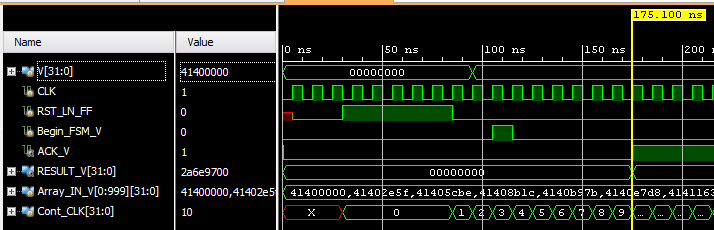
\includegraphics[scale=0.8]{./TEST_CONV_NOM_I.png}
    \rule{35em}{0.5pt}
  \caption[Simulación del circuito de conversión y normalización]{Simulación del circuito de conversión y normalización}
  \label{fig:SIMNORM}
\end{figure}

\section{Simulación y verificación del convertidor-normalizador}

En la implementación de un diseño en hardware, es de suma importancia simular y verificar que este funcione de manera adecuada al comportamiento esperado teóricamente. Para la comprobación de la unidad de conversión-normalización, se realizaron una serie de pruebas en donde se programó una simulación ("testbench") que contiene una prueba con mil valores de entrada, ingresados por medio de un archivo de texto previamente editado con los datos de entrada del comportamiento segun el modelo del panel, las pruebas de esta unidad se realizaron con valores de corriente $ i_{pv}$ y valores de tension $ V_{pv}$. 


  \begin{figure}[H]
  \centering
    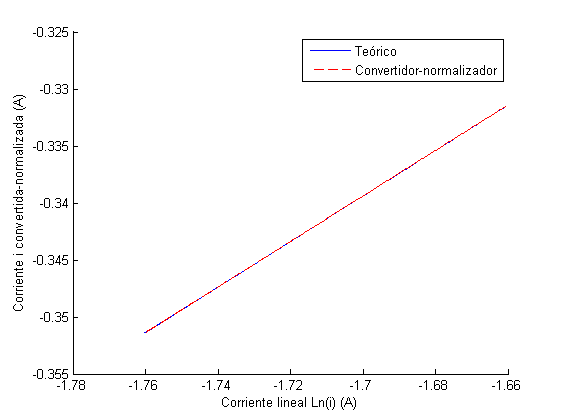
\includegraphics[scale=0.7]{./Convertidor-normalizador_I.png}
    \rule{35em}{0.5pt}
  \caption[Comparación entre la conversión-normalización de corriente $\ i_{pv}$ teórica y del circuito]{Comparación entre la conversión-normalización de corriente $\ i_{pv}$ teórica y del circuito}
  \label{fig:NORMI}
\end{figure}

En la figura \ref{fig:NORMI} se presenta la comparación entre los resultados obtenidos teóricamente y experimentalmente, tomando como datos de entrada  valores de corriente en formato punto flotante y retornando en la salida valores de corriente normalizados y en formato punto fijo. Estos resultados se pueden comparar por medio del porcentaje de error.  

  \begin{figure}[H]
  \centering
    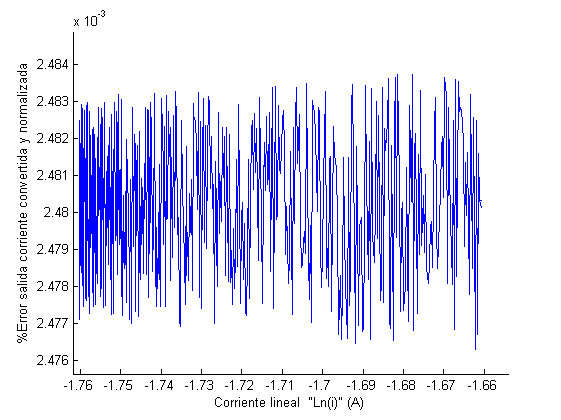
\includegraphics[scale=0.7]{./ERROR_CONV_NORM_I.png}
    \rule{35em}{0.5pt}
  \caption[\%Error entre la conversión-normalización de corriente $\ i_{pv}$ teórica y del circuito]{\%Error entre la conversión-normalización de corriente $\ i_{pv}$ teórica y del circuito}
  \label{fig:ENORMI}
\end{figure}

En la figura \ref{fig:ENORMI} se puede observar el error entre la conversión de la corriente normalizada teórica y experimental, con un error porcentual máximo de 0,0024837\% y un error promedio de 0,002478\% 


  \begin{figure}[H]
  \centering
    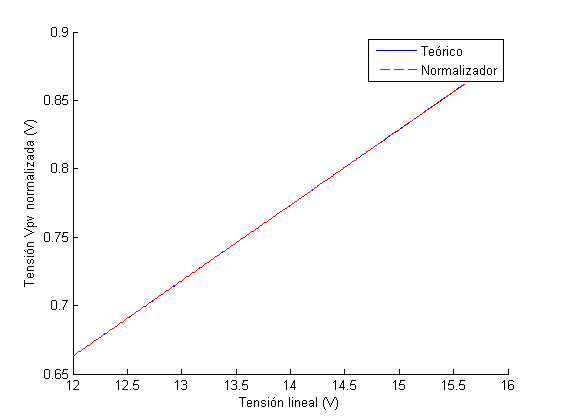
\includegraphics[scale=0.7]{./Normalizador_V.png}
    \rule{35em}{0.5pt}
  \caption[Comparación entre la conversión-normalización de tensión $\ V_{pv}$ teórica y del circuito]{Comparación entre la conversión-normalización de tensión  $\ V_{pv}$ teórica y del circuito}
  \label{fig:NORMV}
\end{figure}


  \begin{figure}[H]
  \centering
    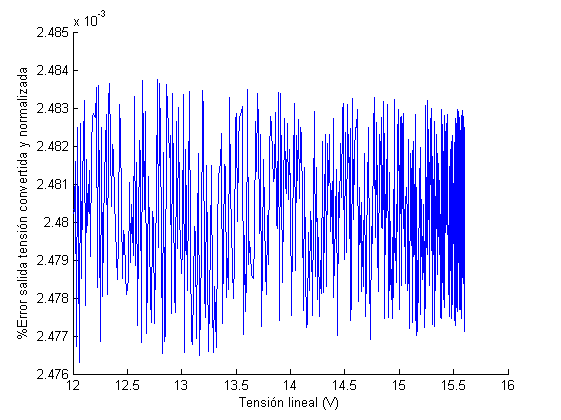
\includegraphics[scale=0.7]{./ERROR_CONV_NORM_V.png}
    \rule{35em}{0.5pt}
  \caption[\%Error entre la conversión-normalización de tensión $\ V_{pv}$ teórica y del circuito]{\%Error entre la conversión-normalización de tensión $\ V_{pv}$ teórica y del circuito}
  \label{fig:ENORMV}
\end{figure}

El análisis utilizado para la conversión-normalización de la corriente se utiliza para los resultados de la tensión, en la figura \ref{fig:NORMV} se muestran los resultados obtenidos con una tension de entrada y su normalizacion tanto teorico como experimental, de la misma manera se puede hacer el calculo del error entre ambas, en la figura \ref{fig:ENORMV} se puede observar el error máximo de 0,0024837\% y un error promedio de 0,002478\%.

Esta unidad contiene muchos bloques combinacionales, por lo que se requieren pocos ciclos de reloj en la maquina de estados para realizar la conversión y la normalización, la maquina de estados finita indica que  se requieren 8 ciclos de reloj para que el resultado sea concluido, con las simulaciones efectuadas al circuito se comprueba como se mostró en la  figura \ref{fig:SIMNORM} 

  \chapter{Sistema de linealización, conversión punto flotante a punto fijo y normalización}

En la implementación del circuito completo se utilizan dos etapas, una para corriente del panel $i_{pv}$ y otra para la tensión del panel $V_{pv}$.

\begin{compactitem}

\item \nt{Corriente $i_{pv}$}: El bloque para la corriente requiere las etapa de linealización, conversión de la salida del linealizador de punto flotante a punto fijo, y un normalizador que da una salida de corriente entre el rango [-1,1].

\item \nt{Tensión $V_{pv}$}: La tension del panel se trabaja de manera lineal, de manera que solo se requiere de un normalizador que contenga la salida entre el intervalo [0,1]. 

\end{compactitem}

\begin{figure}[H]
  \centering
    \includegraphics[scale=0.04]{./Linealizador_normalizador.png}
    \rule{35em}{0.5pt}
  \caption[Sistema de linealización, conversión y normalización de corriente y tensión para un panel fotovoltaico]{Sistema de linealización, conversión y normalización de corriente y tensión para un panel fotovoltaico}
  \label{fig:Sist1}
\end{figure}


El sistema de la figura \ref{fig:Sist1} cuenta con 6 entradas y 4 salidas, estas se describen a continuación. 

Entradas:
\begin{compactitem}

\item \nt{CLK}: Reloj del sistema.
\item \nt{I}: Dato de corriente en formato IEEE 754
\item \nt{V}: Dato de tensión en formato IEEE 754
\item \nt{RST\_LN\_FF}: Reset para las unidades de corriente y tensión. 
\item \nt{Begin\_FSM\_I}: Inicia la máquina de estados del linealizador de corriente. 
\item \nt{Begin\_FSM\_V}: Inicia la máquina de estados de el convertidor punto flotante-punto fijo para la tensión. 

\end{compactitem}
Salidas:

\begin{compactitem}

\item \nt{ACK\_I}: Esta bandera indica que el resultado de las operaciones para la corriente se encuentra listo.  
\item \nt{ACK\_V}: Esta bandera indica que el resultado de las operaciones para la tensión se encuentra listo.  
\item \nt{RESULT\_I}: Resultado de corriente lineal y normalizado en formato punto fijo. 
\item \nt{RESULT\_V}: Resultado de de tensión normalizado en formato punto fijo.

\end{compactitem}

\begin{figure}[H]
  \centering
    \includegraphics[scale=0.05]{./Linealizador_normalizador2.png}
    \rule{35em}{0.5pt}
  \caption[Sistema de linealización-conversión-normalización de corriente y sistema de conversión- normalización de tensión para un panel fotovoltaico]{Sistema de linealización-conversión-normalización de corriente y sistema de conversión- normalización de tensión para un panel fotovoltaico}
  \label{fig:Sist2}
\end{figure}

La figura \ref{fig:Sist2} muestra la distribución de bloques funcionales para la corriente y tensión que proviene del panel fotovoltaico, todos los bloques se encuentran sincronizados con un mismo reloj $ \left(CLK\right)$ para la sección de corriente se realiza primeramente la linealización, iniciando con las señales RST\_LN\_FF y Begin\_FSM\_I y el dato de entrada I (corriente $\ i_{pv}$), una vez ejecutada la operación se envía una señal indicando que el dato esta listo ACK\_LN, esta se conecta a la señal de entrada e inicio del convertidor-normalizador de corriente Begin\_FF, justamente un ciclo de reloj antes de que esta señal de control se envíe, el resultado de la linealización $ \left(RESULT\right)$ esta listo, este está conectado a la entrada F del convertidor-normalizador, la ejecución de este se comprueba con la señal ACK\_I en donde se indica que la conversión-normalización fue realizada y el resultado se encuentra en RESULT\_I (corriente lineal y normalizada en punto fijo  $\ y' $).    

El bloque de tensión funciona de manera similar al de corriente, iniciando con las señales RST\_LN\_FF y Begin\_FSM\_V y el dato de entrada V (tensión $\ V_{pv}$), una vez ejecutada la operación se envía una señal indicando que el dato esta listo ACK\_V, el resultado se despliega en RESULT\_V (tensión normalizada en punto fijo  $\ z' $).

\section{Circuito para realizar las pruebas en Nexys-4}

Para desarrollar las pruebas dentro de la FPGA, se requirió diseñar e implementar un circuito para insertar datos a la entrada del linealizador-normalizador, sean procesados y posteriormente enviados por medio de transmisión serial hacia un computador.  

\begin{figure}[H]
  \centering
    \includegraphics[scale=0.06]{./test.png}
    \rule{35em}{0.5pt}
  \caption[Circuito de prueba para enviar datos por medio de UART desde la nexys-4 hacia un computador]{Circuito de prueba para enviar datos por medio de UART desde la nexys-4 hacia un computador}
  \label{fig:test}
\end{figure}

El diagrama de la figura \ref{fig:test} muestra el diseño del circuito utilizado, en donde se tiene una sección para ingresar 1024 datos, estos son almacenados en una memoria ROM, esta se carga por medio de un archivo de texto que contiene los datos de entrada para el linealizador-normalizador, esta memoria posee un contador para direccionar los 1024 datos. La sección de transmisión posee una unidad UART, esta se utiliza para enviar los resultados de la unidad de linealización-normalización hacia el computador, estos resultados tienen un formato punto fijo de 32 bits, el uart envía únicamente paquetes de 8 bits, por lo que se requiere enviar 4 paquetes por cada resultado, esto se logra por medio de una configuración de un multiplexor 4x1 y un contador, las entradas del multiplexor contienen el resultado dividido en paquetes de 8 bits y el contador selecciona el multiplexor según sea el paquete que se desea enviar. Por ultimo se cuenta con un control para el circuito, este se encarga de llevar la sincronía de los datos, primeramente se realiza una carga en el contador de la memoria ROM, este carga la primera posición de la ROM, posteriormente se inicia el procesamiento por parte de la unidad de linealización-normalización con la señal $\ Begin\_op$, el control espera a que el resultado este listo por medio de la señal ACK, cuando la condición ACK=High, el sistema se encuentra listo para transmitir, el contador del multiplexor selecciona el primer paquete y lo envía, el siguiente paquete se puede transmitir hasta que el modulo UART envié la señal $\ TX\_DONE$, así sucesivamente hasta que se envíen los 4 paquetes, cuando la selección del multiplexor esta en 2b'11 (contador del multiplexor), la señal $\ max\_tick\_mux$ indica al control que debe realizar una cuenta para la dirección de la ROM. Este proceso se repite hasta que la cuenta de las direcciones de la ROM es 1023 y la señal $\ max\_tick\_add = 1 $.
La recepción de datos desde el computador se realizo por medio del un puerto USB y un script realizado en Matlab, este recibe los paquetes de un byte en hexadecimal y los concatena en paquetes de 4 bytes, para formar el dato en 32 bits, posteriormente se convierte a decimal.   

\section{Simulación del sistema de linealización, conversión punto flotante a punto fijo y normalización implementado en hardware}

Este circuito se implementó por medio de la unión de los bloques anteriormente diseñados, implementados y simulados. 

\begin{figure}[H]
  \centering
    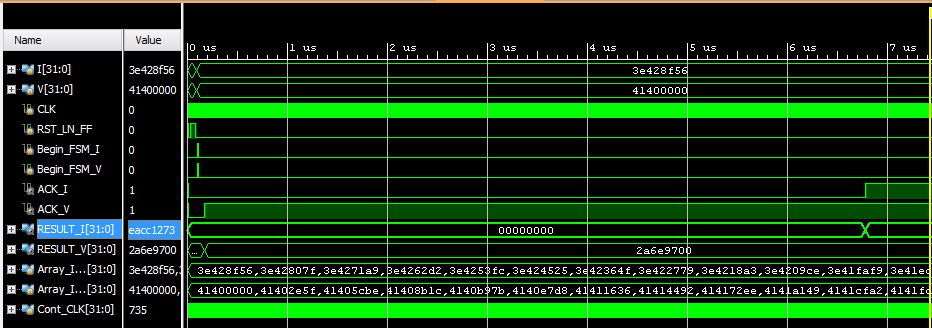
\includegraphics[scale=0.6]{./TEST_LINEALIZADOR_NORMALIZADOR.png}
    \rule{35em}{0.5pt}
  \caption[Simulación del sistema de linealización-conversión-normalización de corriente y sistema de conversión- normalización de tensión para un panel fotovoltaico]{Simulación del sistema de linealización-conversión-normalización de corriente y sistema de conversión- normalización de tensión para un panel fotovoltaico}
  \label{fig:Sim_Sist}
\end{figure}

La simulación básica "behavioral" efectuada por Vivado, verifica el funcionamiento adecuado del circuito a manera de software y de lógica sin embargo no es suficiente ya que se debe realizar la sintesis e implementación en verilog (Hardware), para esto se realizan las simulaciones post-syntesis y post-implementation, tanto del funcionamiento como de los retardos del sistema. La figura \ref{fig:Sim_Sist} muestra la simulación de tiempos posterior a la implementación.

\section{Resultados del sistema de linealización, conversión punto flotante a punto fijo y normalización implementado y verificado en hardware por medio de una FPGA nexys-4}

Las simulaciones para el circuito completo brindan una mejor información acerca del porcentaje de error total obtenido dentro de la conexión de las tres etapas  linealización, conversión y normalización. Se efectuaron las simulaciones de temporización y funcionalidad posterior a la síntesis, obteniendo resultados experimentales para realizar comparación contra los teóricos esperados.      
 
En el capítulo 3 se demostró el funcionamiento del linealizador con 8,12 y 15 iteraciones para el rango de convergencia del algoritmo de CORDIC, en este capítulo se utiliza el mismo principio de verificación, sin embargo se debe contemplar el error del normalizador, por lo que se realizan pruebas y comparaciones similares utilizando como datos de entrada un barrido de 1000 valores ingresados en el modelo teórico del panel fotovoltaico, esto con el fin de observar un comportamiento similar al real, estos valores de corriente son pequeños debido a la diferencia de corrientes y perdidas en el panel fotovoltaico, por lo que los porcentajes de error serán menores, ya que el circuito posee una mejor aproximación en el extremo inferior del intervalo de convergencia del algoritmo CORDIC. La visualización de los resultados obtenidos se realiza de una mejor manera mediante gráficos que indican como se comporta el circuito ante datos de entrada, salida, y porcentaje de error, apartir de los resultados de las simulaciones, se puede analizar la frecuencia de ejecución a la que se obtiene un resultado linealizado-normalizado, esta depende del numero de iteraciones que se utilice, por otro lado se deben sumar los ciclos de cada uno de los bloques funcionales que componen la ruta de ejecución de la corriente este circuito, se detallará de mejor manera en la siguiente sección.
Si tomamos el bloque para la tensión, este solo cuenta con la conversión-normalización y no depende del número de iteraciones por lo que se requieren de 8 ciclos de reloj por cada dato. 

\subsection{Sistema de linealización, conversión y normalización para la corriente $\ i_{pv}$ con 8 iteraciones implementado en una FPGA nexys-4} 
 
A partir de las simulaciones post-síntesis efectuadas por medio de la herramienta Vivado con una aproximación de 8 iteraciones, se puede observar que se requiere de 468 ciclos de reloj para completar la ejecución de un dato, este se compone de 460 ciclos de reloj para el linealizador y 8 ciclos de reloj para el convertidor-normalizador, donde la velocidad de ejecución es de 217kHz con un reloj de sistema de 100MHz.  

\begin{figure}[H]
  \centering
    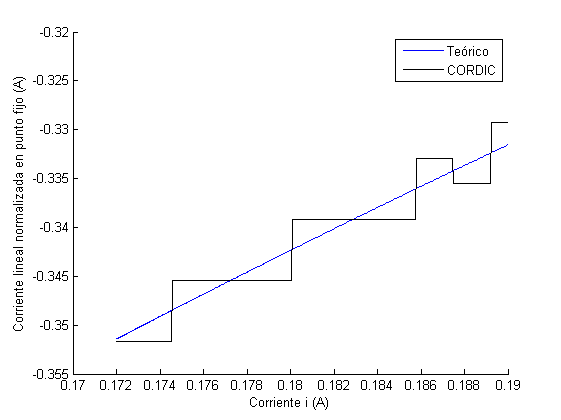
\includegraphics[scale=0.7]{./LINEALIZADOR_NORMALIZADOR_8iter.png}
    \rule{35em}{0.5pt}
  \caption[Comparación entre el valor teórico y el valor obtenido del circuito de linealización-conversión-normalización de corriente con 8 iteraciones en el algoritmo de CORDIC del linealizador]{Comparación entre el valor teórico y el valor obtenido del circuito de linealización-conversión-normalización de corriente con 8 iteraciones en el algoritmo de CORDIC del linealizador}
  \label{fig:LIN_NOR_8}
\end{figure}

\begin{figure}[H]
  \centering
    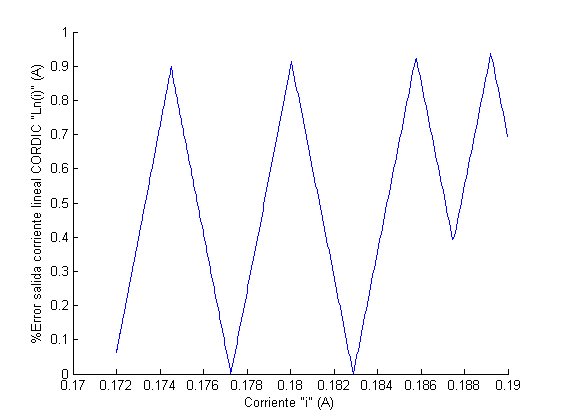
\includegraphics[scale=0.7]{./LINEALIZADOR_NORMALIZADOR_8iter_ERROR.png}
    \rule{35em}{0.5pt}
  \caption[Porcentaje de error entre el valor teórico y el valor obtenido del circuito de linealización-conversión-normalización de corriente con 8 iteraciones en el algoritmo de CORDIC del linealizador]{Porcentaje de error entre el valor teórico y el valor obtenido del circuito de linealización-conversión-normalización de corriente con 8 iteraciones en el algoritmo de CORDIC del linealizador}
  \label{fig:LIN_NOR_8_E}
\end{figure}

En la figura \ref{fig:LIN_NOR_8} se puede observar la comparación entre los datos obtenidos del circuito implementado en una FPGA nexys-4 contra los datos teóricos al realizar la misma función del circuito, debido a que son solo 8 iteraciones el circuito posee un resultados aceptables pero poco exactos, el gráfico muestra que el algoritmo trata de mantenerse cerca de los valores reales, sin embargo posee un comportamiento escalonado, en donde para cierta cantidad de valores de entrada posee un mismo valor de salida constante cercano al valor real. La figura \ref{fig:LIN_NOR_8_E} muestra el porcentaje de error asociado a cada valor de entrada linealizado y normalizado en formato punto fijo, donde el porcentaje de error máximo es de 0,922\% y un porcentaje de error promedio de 0,455\% esto para valores de corriente derivados a partir del modelo teórico del panel fotovoltaico. 
  

\subsection{Sistema de linealización, conversión y normalización para la corriente $\ i_{pv}$ con 12 iteraciones implementado en una FPGA nexys-4} 

Según las simulaciones post-sintesis del circuito con una configuración del algoritmo de CORDIC con 12 iteraciones, se requiere de 668 ciclos de reloj para realizar el procesamiento completo de un dato de entrada, 660 ciclos de reloj son utilizados por el linealizador y 8 ciclos de reloj para el convertidor-normalizador, con una velocidad de ejecución de 151kHz, utilizando un reloj de sistema de 100MHz.   

\begin{figure}[H]
  \centering
    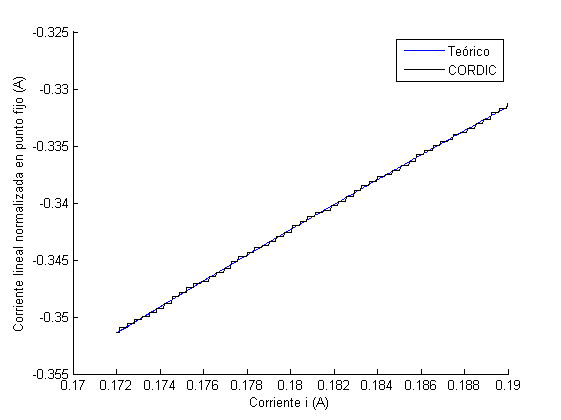
\includegraphics[scale=0.7]{./LINEALIZADOR_NORMALIZADOR_12iter.png}
    \rule{35em}{0.5pt}
  \caption[Comparación entre el valor teórico y el valor obtenido del circuito de linealización-conversión-normalización de corriente con 12 iteraciones en el algoritmo de CORDIC del linealizador]{Comparación entre el valor teórico y el valor obtenido del circuito de linealización-conversión-normalización de corriente con 12 iteraciones en el algoritmo de CORDIC del linealizador}
  \label{fig:LIN_NOR_12}
\end{figure}


\begin{figure}[H]
  \centering
    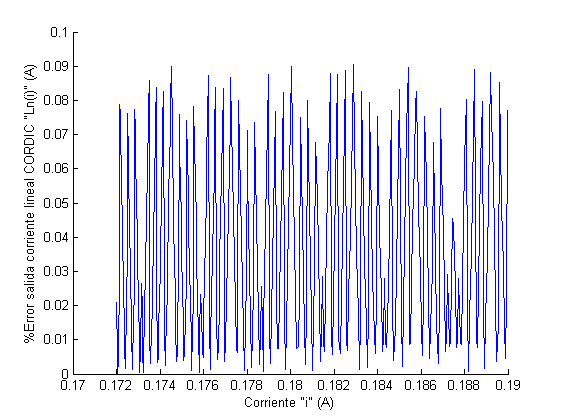
\includegraphics[scale=0.7]{./LINEALIZADOR_NORMALIZADOR_12iter_ERROR.png}
    \rule{35em}{0.5pt}
  \caption[Porcentaje de error entre el valor teórico y el valor obtenido del circuito de linealización-conversión-normalización de corriente con 12 iteraciones en el algoritmo de CORDIC del linealizador]{Porcentaje de error entre el valor teórico y el valor obtenido del circuito de linealización-conversión-normalización de corriente con 12 iteraciones en el algoritmo de CORDIC del linealizador}
  \label{fig:LIN_NOR_12_E}
\end{figure}

En la figura \ref{fig:LIN_NOR_12} se puede observar la comparación entre los datos obtenidos experimentalmente contra los datos teóricos al realizar la misma función del circuito, el uso de 12 iteraciones brinda una mejor exactitud contra 8 iteraciones, se puede observar que se presenta una mayor suavidad en la curva, sin embargo siempre se presenta un comportamiento escalonado pero con un valor mas cercano a la curva real. La figura \ref{fig:LIN_NOR_12_E} muestra el porcentaje de error asociado a cada valor de entrada linealizado con 12 iteraciones y normalizado en formato punto fijo, donde el porcentaje de error máximo es de 0,0897\% y un porcentaje de error promedio de 0,0345\% esto para valores de corriente derivados a partir del modelo teórico del panel fotovoltaico.


\subsection{Sistema de linealización, conversión y normalización para la corriente $\ i_{pv}$ con 15 iteraciones implementado en una FPGA nexys-4} 

En el sistema del panel es de suma importancia el tiempo de muestreo según sea la frecuencia del panel, esto implica velocidad de ejecución dentro del cálculo, se logró determinar que con 15 iteraciones se obtienen resultados con muy buena exactitud,sin embargo el tiempo de ejecución aumenta a 826 ciclos de reloj, tomando en cuenta que 818 ciclos son requeridos por el linealizador y 8 ciclos de reloj para la conversión de formato IEEE 754 a punto fijo y normalización, en donde la velocidad de ejecución es de 121kHz con un reloj de sistema de 100MHz.  


\begin{figure}[H]
  \centering
    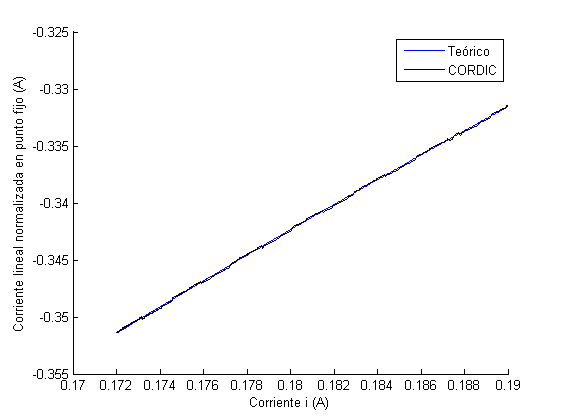
\includegraphics[scale=0.7]{./LINEALIZADOR_NORMALIZADOR_15iter.png}
    \rule{35em}{0.5pt}
  \caption[Comparación entre el valor teórico y el valor obtenido del circuito de linealización-conversión-normalización de corriente con 15 iteraciones en el algoritmo de CORDIC del linealizador]{Comparación entre el valor teórico y el valor obtenido del circuito de linealización-conversión-normalización de corriente con 15 iteraciones en el algoritmo de CORDIC del linealizador}
  \label{fig:LIN_NOR_15}
\end{figure}

\begin{figure}[H]
  \centering
    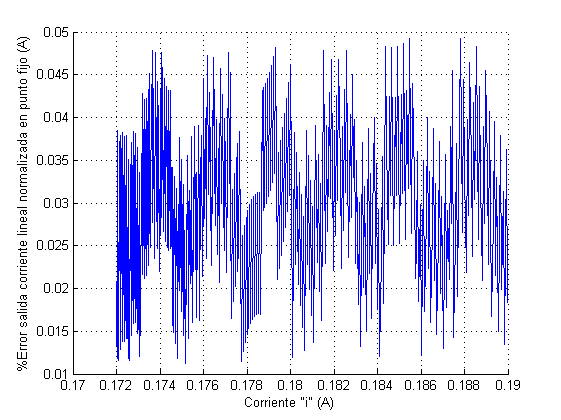
\includegraphics[scale=0.7]{./LINEALIZADOR_NORMALIZADOR_15iter_ERROR.png}
    \rule{35em}{0.5pt}
  \caption[Porcentaje de error entre el valor teórico y el valor obtenido del circuito de linealización-conversión-normalización de corriente con 15 iteraciones en el algoritmo de CORDIC del linealizador]{Porcentaje de error entre el valor teórico y el valor obtenido del circuito de linealización-conversión-normalización de corriente con 15 iteraciones en el algoritmo de CORDIC del linealizador}
  \label{fig:LIN_NOR_15_E}
\end{figure}

Con 15 iteraciones el valor experimental es muy similar al valor teórico, como se observa en la figura \ref{fig:LIN_NOR_15}, y se puede comprobar en la figura \ref{fig:LIN_NOR_15_E} donde se muestra que el porcentaje de error es muy cercano a cero, con un valor máximo de 0,0483\% y un error promedio de 0,0292\% esto para valores de corriente derivados a partir del modelo teórico del panel fotovoltaico.

El sistema de optimización se utilizará en un panel fotovoltaico que posee una frecuencia de 100kHz, es decir que el sistema de optimización debe realizar un cálculo completo velocidad mayor que el panel, aproximadamente el sistema de linealización y normalización toma un 40\% del total del tiempo de ejecución del sistema de optimización. Según lo anterior para realizar el cálculo en el tiempo indicado, el linealizador deberá utilizar 8 iteraciones.    


\section{Recursos utilizados}


\begin{table}[H]
\centering
\caption{Resumen del reporte post implementación del uso de dispositivos generado por la herramienta Vivado.}
\label{Table:Recursos}
\begin{tabular}{|c|c|c|c|c|c|}
\hline
Recurso & Utilizados  & Disponibles & Utilizados\%   \\ \hline

\begin{tabular}[c]{@{}c@{}} LUT
\end{tabular}  & 1017 &  63400   & 1.60      \\ \hline

\begin{tabular}[c]{@{}c@{}} FF
\end{tabular} & 912 & 126800   & 0.72         \\ \hline

\begin{tabular}[c]{@{}c@{}} DSP 
\end{tabular} & 4 & 240   & 1.67       \\ \hline

\begin{tabular}[c]{@{}l@{}} IO
\end{tabular} & 134 & 210   & 63.81     \\ \hline

\begin{tabular}[c]{@{}l@{}} BUFG
\end{tabular} & 1 & 32   & 3.12   \\ \hline

\end{tabular}
\end{table}

En la tabla \ref{Table:Recursos} se muestra el uso de recursos para la implementación el circuito completo en la Nexys4, el máximo recurso utilizado son los puertos I/O debido a que se requieren 32 bits en cada entrada I,V y 32 bits en cada salida RESULT\_I , RESULT\_V, sin embargo el uso de los demás recursos es sumamente bajo, el uso de los I/O se reducirá debido a que este circuito se deben acoplar a otro bloques del sistema de optimización.
  
\section{Reporte de tiempos}

Dentro del reporte de tiempos se analizan las peores rutas "ruta critica", para un buen diseño se requiere de slacks positivos, en el caso de "setup" un slack positvo indica que el dato llega a tiempo antes de ser utilizado, en el caso del "hold" indica que se mantiene por el tiempo adecuado antes de ser procesado por otro bloque, si ambos slacks son cero, el diseño esta en el limite y puede ser un poco arriesgado en sincronización. En la tabla \ref{Table:Tiempos} se muestran los valores obtenidos para los slacks del circuito del linealizador-normalizador.    

\begin{table}[H]
\centering
\caption{Resumen del reporte post implementación de tiempos del circuito completo, a partir de la herramienta Vivado.}
\label{Table:Tiempos}
\begin{tabular}{|c|c|c|}
\hline
Peor slack de todas las rutas & tiempo $ \left(ns\right) $      \\ \hline

\begin{tabular}[c]{@{}c@{}} Setup
\end{tabular}  & 0.459         \\ \hline

\begin{tabular}[c]{@{}c@{}} Hold
\end{tabular}  & 0.109          \\ \hline

\begin{tabular}[c]{@{}c@{}} Pulse width
\end{tabular}  & 4.5         \\ \hline


\end{tabular}
\end{table}

\section{Consumo de potencia}
Con la ayuda de las herramientas de análisis de potencia de Vivado, se pudo obtener los resultados que pertenecen al consumo de potencia, tanto estática como dinámica. En la tabla \ref{Table:Potencia1} se muestra el valor para cada consumo, y el total. 

\begin{table}[H]
\centering
\caption{Resumen del reporte post implementación de la potencia estática, dinámica y total, de la herramienta Vivado.}
\label{Table:Potencia1}
\begin{tabular}{|c|c|c|}
\hline
Potencia  & Consumo de potencia $ \left(mW\right) $      \\ \hline

\begin{tabular}[c]{@{}c@{}} Dinámica
\end{tabular}  & 11         \\ \hline

\begin{tabular}[c]{@{}c@{}} Estática
\end{tabular}  & 91          \\ \hline

\begin{tabular}[c]{@{}c@{}} Total
\end{tabular}  & 102         \\ \hline



\end{tabular}
\end{table}


Para los recursos utilizados se puede realizar un estudio de consumo de potencia dinámica, estos resultados se muestran en la tabla \ref{Table:Potencia2} donde el mayor consumo de potencia se presenta por parte del reloj del sistema y señales, las señales que poseen un valor de cero no se refieren a un consumo nulo, si no que es relativamente pequeño en comparación con las señales mas criticas.

\begin{table}[H]
\centering
\caption{Resumen del reporte generado por la herramienta Vivado que indica el consumo de potencia de diversos elementos. }
\label{Table:Potencia2}
\begin{tabular}{|c|c|c|c|c|c|c|}
\hline
On-chip $ \left(mW\right)$ & Consumo de potencia $ \left(mW\right) $      \\ \hline

\begin{tabular}[c]{@{}c@{}} Clocks
\end{tabular}  & 4          \\ \hline

\begin{tabular}[c]{@{}c@{}} Signals
\end{tabular}  & 4          \\ \hline

\begin{tabular}[c]{@{}c@{}} Logic
\end{tabular}  & 3          \\ \hline

\begin{tabular}[c]{@{}c@{}} DSP
\end{tabular}  & 0          \\ \hline

\begin{tabular}[c]{@{}c@{}} I/O
\end{tabular}  & 0          \\ \hline


\end{tabular}
\end{table}
  %\chapter{Resultados y análisis}

En tesis formales en este capítulo se exponen los diseños experimentales
realizados para comprobar el funcionamiento correcto del sistema. Por ejemplo,
si se realiza algún sistema con reconocimiento de patrones, usualmente esta
sección involucra las llamadas \emph{matrices de confusión} donde se compactan
las estadísticas de reconocimiento alcanzadas. En circuitos de hardware,
experimentos para determinar variaciones contra ruido, etc. También pueden
ilustrarse algunos resultados concretos como ejemplo del funcionamiento de los
algoritmos. Puede mostrar por medio de experimentos ventajas, desventajas,
desempeño de su algoritmo, o comparaciones con otros algoritmos.

Recuerde que debe minimizar los ``saltos'' que el lector deba hacer en su
documento. Por tanto, usualmente el análisis se coloca junto a tablas y figuras
presentadas, y debe tener un orden de tal modo que se observe cómo los
objetivos específicos y el objetivo general del proyecto se han cumplido.

  \chapter{Conclusiones}

Las conclusiones no son un resumen de lo realizado sino a lo que ha llevado el
desarrollo del proyecto, no perdiendo de vista los objetivos planteados desde
el principio y los resultados obtenidos.  En otras palabras, qué se concluye o
a qué se ha llegado después de realizado el proyecto de graduación.  Un error
común es ``concluir'' aspectos que no se desarrollaron en la tesis, como
observaciones o afirmaciones derivadas de la teoría directamente.  Esto último
debe evitarse.

Es usual concluir con lo que queda por hacer, o sugerencias para mejorar los
resultados.



  %----------------------------------------------------------------------------
  % literature
  \bibliographystyle{sty/plainurl} % for english documents
  %\bibliography{literatura}
  %\bibliography{referencias}
  \chapter{bibliográficas}

[1] Suskis, Pavels, and Ilya Galkin. "Enhanced photovoltaic panel model for MATLAB-simulink environment considering solar cell junction capacitance." Industrial Electronics Society, IECON 2013-39th Annual Conference of the IEEE. IEEE, 2013.

[2] González-Longatt, Francisco M. "Model of photovoltaic module in Matlab." II CIBELEC 2005 (2005): 1-5.

[3] C. Meza, R. Ortega, "Control and estimation scheme for PV central inventers", in 24th International Conference on information, Comunication and Automation Technologies, Nov, 2013 

[4] Chiang, Ching-Tsan, Tung-Sheng Chiang, and Hou-Sheng Huang. "Modeling a photovoltaic power system by CMAC-GBF." Photovoltaic Energy Conversion, 2003. Proceedings of 3rd World Conference on. Vol. 3. IEEE, 2003.

[5] Ibrahim, Muhammad Nasir, et al. "Hardware Implementation of Math Module Based on CORDIC Algorithm Using FPGA." Parallel and Distributed Systems (ICPADS), 2013 International Conference on. IEEE, 2013.

[6] Walther, John S. "A unified algorithm for elementary functions." Proceedings of the May 18-20, 1971, spring joint computer conference. ACM, 1971.

[7] Llamocca-Obregón, Daniel R., and Carla P. Agurto-Ríos. "A fixed-point implementation of the expanded hyperbolic CORDIC algorithm." Latin American applied research 37.1 (2007): 83-91.

[8] Whitehead, Nathan, and Alex Fit-Florea. "Precision and performance: Floating point and IEEE 754 compliance for NVIDIA GPUs." rn (A+ B) 21 (2011): 1-1874919424.

[9] Bello, C., et al. "Relevador portátil de curvas IV de paneles fotovoltaicos como herramienta de diagnostico in situ de sistemas de generación fotovoltaica." Avances en Energías Renovables y Medio Ambiente 13 (2009): 77-83.

[10] Raygoza, Juan José, et al. "Implementación en hardware de un sumador de punto flotante basado en el estándar IEEE 754-2008." e-Gnosis 7 (2009).

[11] Bube, Richard. Fundamentals of solar cells: photovoltaic solar energy conversion. Elsevier, 2012.

[12] Boudabous, Anis, et al. "Implementation of hyperbolic functions using CORDIC algorithm." Microelectronics, 2004. ICM 2004 Proceedings. The 16th International Conference on. IEEE, 2004.

[13] Mano, M. Morris. Arquitectura de computadoras. Pearson Educación, 1994.

[14] Floyd, Thomas L. Fundamentos de sistemas digitales. Vol. 7. Prentice Hall, 2006.
  %----------------------------------------------------------------------------

  %----------------------------------------------------------------------------
  \appendix
  %----------------------------------------------------------------------------

  %\chapter{Demostración del teorema de Nyquist}

El título anterior es solo un ejemplo ilustrativo.  Éste teorema no ameritaría
un apéndice pues es parte normal del currículum de Electrónica, pero apéndices
usualmente involucran aspectos de esta índole, que se salen de la línea de la
tesis, pero que es conveniente incluir por completitud.

Los anexos contienen toda información adicional que se considere pertinente
agregar, como manuales de usuario, demostraciones matemáticas que se salen de
la línea principal de la tesis, pero que pueden considerarse parte de los
resultados del trabajo.


  %----------------------------------------------------------------------------
  \backmatter
  %----------------------------------------------------------------------------

  \printindex                % insert index into document. Don't forget to call
                             % "makeindex filename" first.
\end{document}
